\documentclass[11pt,a4paper]{article}

% Image mode: pdf.
% Image paths stay relative. In PDF mode, place same-basename PDF conversions
% of the chapter SVG files in the assets/ directory beside this source.

\usepackage{iftex}
\ifPDFTeX
  \PackageError{handout}{This template requires XeTeX or Tectonic}{Compile with xelatex or tectonic.}
\fi

\usepackage[a4paper,top=18mm,bottom=20mm,left=20mm,right=20mm,headsep=6mm]{geometry}
\usepackage{fontspec}
\usepackage{xeCJK}
\usepackage{amsmath}
\usepackage{unicode-math}

% Font settings are intentionally visible in the generated .tex file.
% These defaults target the macOS machine used for the released PDF.
% Change the family names when compiling on another system.
\setmainfont{Songti TC}
\setsansfont{Heiti TC}
\setmonofont{Menlo}
\setCJKmainfont{Songti TC}
\setCJKsansfont{Heiti TC}
\setCJKmonofont{Heiti TC}
\setmathfont{STIX Two Math}
\XeTeXlinebreaklocale "zh"
\XeTeXlinebreakskip=0pt plus 1pt

\usepackage{xcolor}
\definecolor{HandoutBlue}{HTML}{215A91}
\definecolor{HandoutBlueLight}{HTML}{EEF5FC}
\definecolor{HandoutGreen}{HTML}{39715A}
\definecolor{HandoutGreenLight}{HTML}{EFF8F3}
\definecolor{HandoutGold}{HTML}{8A641C}
\definecolor{HandoutGoldLight}{HTML}{FFF8E8}
\definecolor{HandoutInk}{HTML}{253142}
\definecolor{HandoutMuted}{HTML}{667085}

\usepackage{graphicx}
\makeatletter
% Pandoc 3 emits an accessibility `alt` key for raster/PDF images. Older
% graphicx releases do not know that key, so accept it without changing layout.
\@ifundefined{KV@Gin@alt}{\define@key{Gin}{alt}{}}{}
\newsavebox\pandoc@box
\newcommand*\pandocbounded[1]{%
  \sbox\pandoc@box{#1}%
  \Gscale@div\@tempa{\textheight}{\dimexpr\ht\pandoc@box+\dp\pandoc@box\relax}%
  \Gscale@div\@tempb{\linewidth}{\wd\pandoc@box}%
  \ifdim\@tempb\p@<\@tempa\p@\let\@tempa\@tempb\fi
  \ifdim\@tempa\p@<\p@\scalebox{\@tempa}{\usebox\pandoc@box}%
  \else\usebox{\pandoc@box}%
  \fi
}
\makeatother
\usepackage{float}
\floatplacement{figure}{H}
% Pandoc uses LTcaptype=none for uncaptioned longtables. The caption package
% expects that name to exist as a counter even though it is never displayed.
\newcounter{none}
\usepackage{caption}
\captionsetup[figure]{labelformat=empty,labelsep=none,font=small}

\usepackage{booktabs,longtable,array,calc}
\usepackage{etoolbox}
\makeatletter
\patchcmd\longtable{\par}{\if@noskipsec\mbox{}\fi\par}{}{}
\makeatother

\usepackage[most]{tcolorbox}
\tcbuselibrary{breakable,skins}
\newtcolorbox{HandoutLearningMap}{
  enhanced,breakable,colback=HandoutBlueLight,colframe=HandoutBlue,
  boxrule=0.8pt,arc=1.5mm,left=3mm,right=3mm,top=2mm,bottom=2mm,
  before skip=8pt,after skip=10pt
}
\newtcolorbox{HandoutWorkedExample}{
  enhanced,breakable,colback=HandoutGreenLight,colframe=HandoutGreen,
  boxrule=0.65pt,arc=1.5mm,left=3mm,right=3mm,top=2mm,bottom=2mm,
  before skip=8pt,after skip=10pt
}
\newtcolorbox{HandoutSelfCheck}{
  enhanced,breakable,colback=HandoutGoldLight,colframe=HandoutGold,
  boxrule=0.65pt,arc=1.5mm,left=3mm,right=3mm,top=2mm,bottom=2mm,
  before skip=8pt,after skip=10pt
}

\usepackage{titlesec}
\titleformat{\section}{\sffamily\bfseries\Large\color{HandoutBlue}}{}{0pt}{}
\titleformat{\subsection}{\sffamily\bfseries\large\color{HandoutInk}}{}{0pt}{}
\titleformat{\subsubsection}{\sffamily\bfseries\normalsize\color{HandoutInk}}{}{0pt}{}
\titlespacing*{\section}{0pt}{1.4em}{0.55em}
\titlespacing*{\subsection}{0pt}{1.15em}{0.45em}
\titlespacing*{\subsubsection}{0pt}{0.9em}{0.35em}
\setcounter{secnumdepth}{-\maxdimen}

\usepackage{hyperref}
\usepackage{bookmark}
\IfFileExists{xurl.sty}{\usepackage{xurl}}{}
\urlstyle{same}
\hypersetup{
  colorlinks=true,
  linkcolor=HandoutBlue,
  urlcolor=HandoutBlue,
  citecolor=HandoutBlue,
  pdftitle={選化I-3 溶液的性質},
  pdfsubject={化學},
  pdfcreator={Pandoc with the HighSchooContent LaTeX template}
}

\setlength{\parindent}{0pt}
\setlength{\parskip}{0.55em plus 0.15em minus 0.1em}
\setlength{\emergencystretch}{3em}
\setlength{\LTpre}{0.5em}
\setlength{\LTpost}{0.5em}
\renewcommand{\arraystretch}{1.18}
\providecommand{\tightlist}{%
  \setlength{\itemsep}{0pt}\setlength{\parskip}{0pt}}
\pagestyle{plain}


\begin{document}

\begin{tcolorbox}[
  enhanced,colback=white,colframe=HandoutBlue,boxrule=1.1pt,arc=2mm,
  borderline west={3pt}{0pt}{HandoutBlue},left=5mm,right=4mm,top=4mm,bottom=4mm
]
{\sffamily\small\bfseries\color{HandoutBlue}學生講義}\par
{\sffamily\bfseries\LARGE\color{HandoutInk}選化I-3 溶液的性質}\par
\vspace{0.35em}{\large 由粒子數、分子間作用力與相平衡，連結濃度、蒸氣壓、沸點、凝固點與滲透壓}\par
\vspace{0.45em}{\small\color{HandoutMuted}%
科目：化學
\quad 課程：普通高中選修化學 I
\quad 版本：學生版｜核心＋理解
\quad 校訂：2026-08-29
}\par
\vspace{0.25em}{\small\color{HandoutMuted}範圍：現行選修化學 I 第三章主線；涵蓋物質鑑定與溶液、濃度表示、亨利定律、蒸氣壓與濕度、拉午耳定律、沸點上升、凝固點下降、滲透壓、凡特何夫因數與凝固點實驗}\par
\end{tcolorbox}


溶液是微觀粒子均勻混合的單一相。配方要用濃度說明溶質與溶劑的比例；密閉容器中的蒸發、凝結與氣體溶解要用動態平衡說明；沸點、凝固點與滲透壓則反映溶劑粒子在溶質存在時的化學勢改變。

本章的實際用途包含藥物與點滴配方、環境氣體濃度、氣水與潛水安全、濕度控制、蒸餾分離、汽車冷卻液、食品冷凍、醫療滲透壓與淡化海水。應用邊界由溫度、壓力、稀薄程度、粒子互作用與半透膜選擇性決定。計算時先確定「數了哪種粒子」與「分母代表哪個整體」，再核對這些條件。

\begin{HandoutLearningMap}

\subsection{本章問題與能力}\label{ux672cux7ae0ux554fux984cux8207ux80fdux529b}

\begin{enumerate}
\def\labelenumi{\arabic{enumi}.}
\tightlist
\item
  如何選擇物理性質或化學證據鑑定物質，並利用溶解度差進行分離？
\item
  質量百分率、ppm、莫耳分率、體積莫耳濃度與重量莫耳濃度各以什麼為分母？
\item
  亨利定律如何解釋氣水開瓶、潛水減壓與水體溶氧？
\item
  動態平衡如何建立飽和蒸氣壓，並連到沸點、相對濕度與露點？
\item
  拉午耳定律如何從液相組成求各成分分壓、總壓與氣相組成？
\item
  難揮發性溶質為何同時造成沸點上升、凝固點下降與滲透壓？
\item
  電解質的解離如何用凡特何夫因數納入依數性，測得值又能提供什麼粒子證據？
\end{enumerate}

\end{HandoutLearningMap}

\section{1. 物質的鑑定與溶液}\label{ux7269ux8ceaux7684ux9451ux5b9aux8207ux6eb6ux6db2}

\subsection{1.1 鑑定證據、溶解與混合}\label{ux9451ux5b9aux8b49ux64daux6eb6ux89e3ux8207ux6df7ux5408}

\textbf{物質鑑定}是把未知樣品的可量測性質與參考資料比對，並用足以排除其他候選物的證據得出結論。單一性質可能由多種物質共有，因此可依序組合：

\begin{itemize}
\tightlist
\item
  物理證據：顏色、狀態、密度、熔點、沸點、折射率、溶解度、溶液導電度與光譜。
\item
  化學證據：與特定試劑反應所生的沉澱、氣體、顏色、pH 或氧化還原變化。
\item
  空白組、已知對照組與重複測量：用來確認訊號來自樣品，並估計變異。
\end{itemize}

\textbf{溶液}是溶質粒子以分子、離子或原子尺度均勻分散在溶劑中的單一相混合物。組成比例可在一定範圍內改變，因此溶液沒有單一化學式。溶解過程要同時考慮分開原有的溶質--溶質與溶劑--溶劑作用力，以及形成新的溶質--溶劑作用力。能量變化與粒子分散傾向共同決定溶解是否有利。

水與乙醇混合後體積小於兩者體積和，且溫度上升，證明混合後的粒子排列與交互作用已改變。高精度配方以容量瓶配至最終體積。

\textbf{分離}利用成分的性質差。例如加入只溶解其中一成分的溶劑，可先溶解、過濾，再從濾液回收溶質。設計時同時檢查溶解度差、回收率、溶劑危害與廢液處理。

\begin{HandoutWorkedExample}

\subsection{示範 1｜以連續證據鑑定無色水溶液}\label{ux793aux7bc4-1ux4ee5ux9023ux7e8cux8b49ux64daux9451ux5b9aux7121ux8272ux6c34ux6eb6ux6db2}

三種候選物是 \(NaCl(aq)\)、葡萄糖水溶液與稀 \(HCl(aq)\)。未知液可導電，pH 紙呈強酸性，加入 \(AgNO_3(aq)\) 得白色沉澱。判定未知物。

導電顯示溶液中有可移動離子，排除主要以分子存在的葡萄糖溶液。強酸性支持 \(HCl\) 而不支持中性 \(NaCl\) 溶液。白色沉澱由

\[
Ag^+(aq)+Cl^-(aq)\rightarrow AgCl(s)
\]

證明氯離子存在。「酸性＋氯離子」共同指向 \(HCl(aq)\)。若樣品可能含多種溶質，還需增加定量或光譜證據才能說明完整組成。

\end{HandoutWorkedExample}

\begin{HandoutWorkedExample}

\subsection{示範 2｜用溶解度差設計分離流程}\label{ux793aux7bc4-2ux7528ux6eb6ux89e3ux5ea6ux5deeux8a2dux8a08ux5206ux96e2ux6d41ux7a0b}

固體混合物由食鹽與細沙組成。寫出可分別回收兩者的步驟。

\begin{enumerate}
\def\labelenumi{\arabic{enumi}.}
\tightlist
\item
  加入適量水並攪拌：食鹽在水中溶解度大，細沙很小。
\item
  過濾：濾渣為細沙，用少量水洗滌可移除表面食鹽溶液。
\item
  乾燥濾渣：回收細沙。
\item
  蒸發濾液中的水，使食鹽結晶：利用溶劑與溶質的揮發性差。
\end{enumerate}

若要比較回收率，分別秤量乾燥產物，並用初始樣品建立質量帳。洗滌水太多會增加後續蒸發量，太少則使細沙夾帶食鹽。

\end{HandoutWorkedExample}

\subsection{1.2 濃度的分母}\label{ux6fc3ux5ea6ux7684ux5206ux6bcd}

濃度是溶質量與指定整體的比。各定義的差別主要在分母：

\[
\begin{aligned}
\text{質量百分率}&=\frac{m_{solute}}{m_{solution}}\times100\%,\\
\text{體積百分率}&=\frac{V_{solute}}{V_{solution}}\times100\%,\\
ppm&=\frac{m_{solute}}{m_{solution}}\times10^6,\\
X_i&=\frac{n_i}{\sum_j n_j},\\
C_M&=\frac{n_{solute}}{V_{solution}(\mathrm L)},\\
C_m&=\frac{n_{solute}}{m_{solvent}(\mathrm{kg})}.
\end{aligned}
\]

\(C_M\) 常簡寫為 M，\(C_m\) 常簡寫為 m。在密度接近 \(1.00\ \mathrm{kg\,L^{-1}}\) 的極稀水溶液中，\(1\ \mathrm{mg\,L^{-1}}\approx1\ \mathrm{ppm}\)；正式定義仍是質量比。\(C_M\) 以溶液體積為分母，因此受溫度造成的體積變化影響；質量百分率、莫耳分率與 \(C_m\) 由質量或莫耳數建立，密閉系統內不因熱膨脹直接改變。

\begin{figure}
\centering
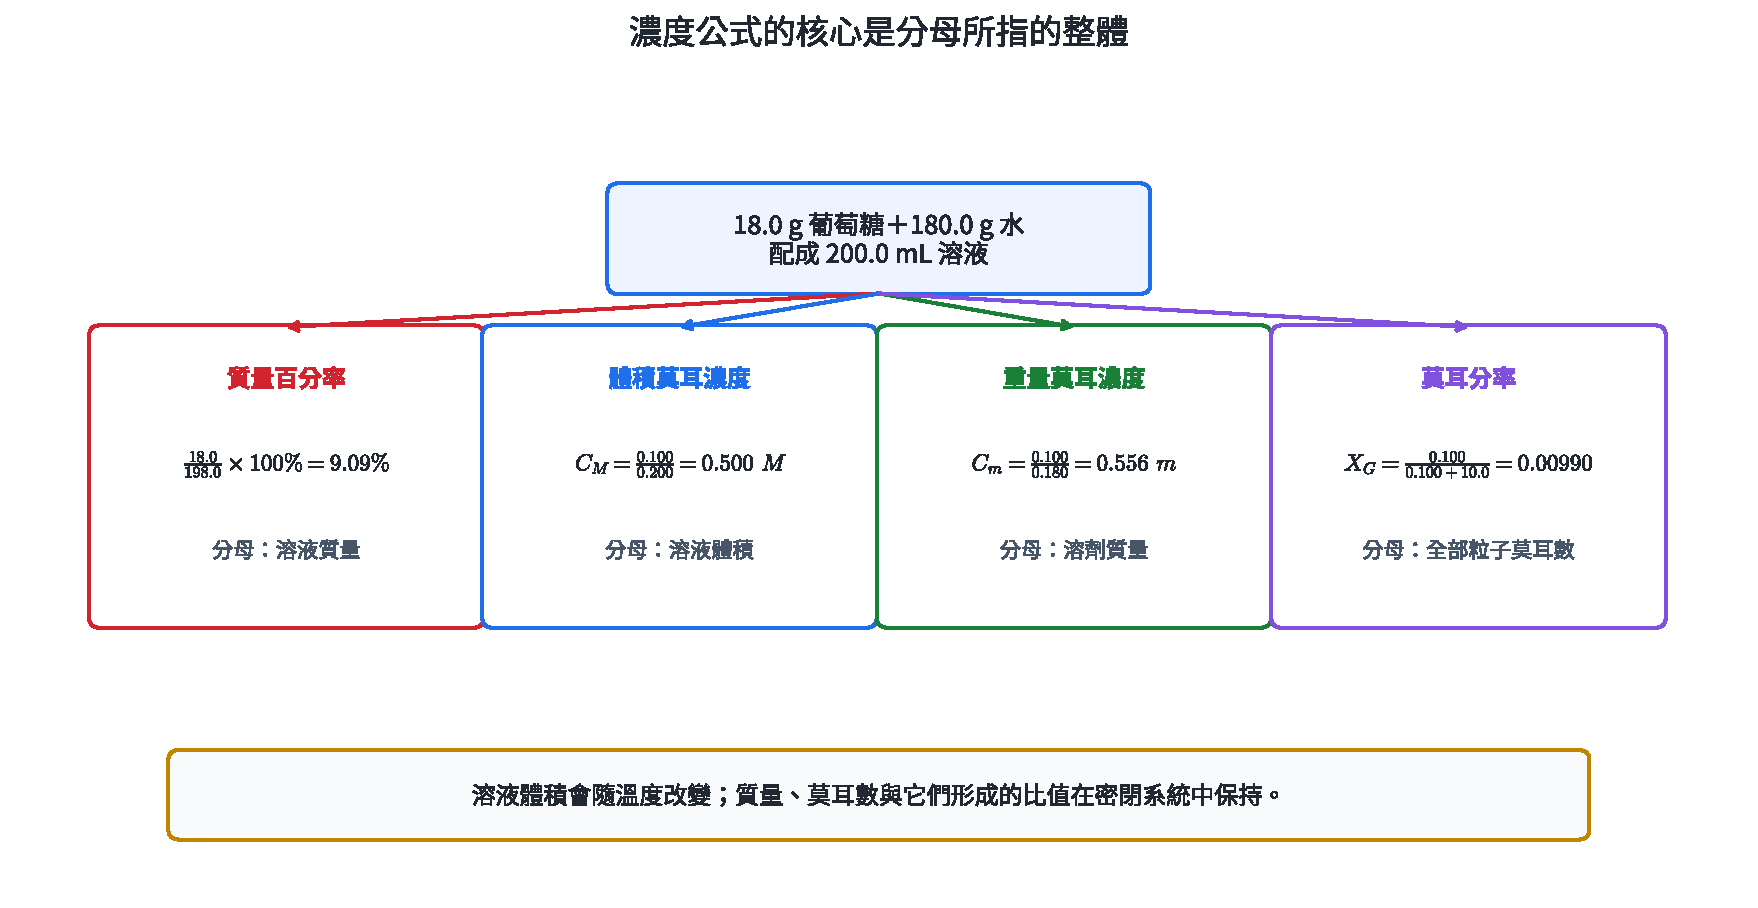
\includegraphics[width=0.98\linewidth,height=\textheight,keepaspectratio,alt={圖 1｜同一份葡萄糖溶液的四種濃度；溶質量相同，分母分別是溶液質量、溶液體積、溶劑質量與全部莫耳數。}]{assets/選化I-3-濃度分母與轉換.pdf}
\caption{圖 1｜同一份葡萄糖溶液的四種濃度；溶質量相同，分母分別是溶液質量、溶液體積、溶劑質量與全部莫耳數。}
\end{figure}

\begin{HandoutWorkedExample}

\subsection{示範 3｜同一溶液的多種濃度}\label{ux793aux7bc4-3ux540cux4e00ux6eb6ux6db2ux7684ux591aux7a2eux6fc3ux5ea6}

\(18.0\ \mathrm g\) 葡萄糖溶於 \(180.0\ \mathrm g\) 水，溶液體積 \(200.0\ \mathrm{mL}\)。取 \(M(\text{葡萄糖})=180.0\ \mathrm{g\,mol^{-1}}\)、\(M(H_2O)=18.0\ \mathrm{g\,mol^{-1}}\)，求質量百分率、\(C_M\)、\(C_m\) 與葡萄糖莫耳分率。

\[
n_G=0.100\ \mathrm{mol},\qquad n_W=10.0\ \mathrm{mol}.
\]

\[
\begin{aligned}
\text{質量百分率}&=\frac{18.0}{198.0}\times100\%=9.09\%,\\
C_M&=\frac{0.100}{0.2000}=0.500\ \mathrm{mol\,L^{-1}},\\
C_m&=\frac{0.100}{0.1800}=0.556\ \mathrm{mol\,kg^{-1}},\\
X_G&=\frac{0.100}{0.100+10.0}=0.00990.
\end{aligned}
\]

四個數值的互換路徑是先還原這份溶液的質量、體積與莫耳數，再換用目標分母。

\end{HandoutWorkedExample}

\begin{HandoutWorkedExample}

\subsection{示範 4｜稀釋與混合的溶質帳}\label{ux793aux7bc4-4ux7a00ux91cbux8207ux6df7ux5408ux7684ux6eb6ux8ceaux5e33}

將 \(250.0\ \mathrm{mL}\)、\(0.400\ \mathrm M\) \(NaCl(aq)\) 與 \(150.0\ \mathrm{mL}\)、\(0.200\ \mathrm M\) \(NaCl(aq)\) 混合，假設體積可加成，求混合後濃度。

\[
n_{total}=(0.400)(0.2500)+(0.200)(0.1500)=0.130\ \mathrm{mol}.
\]

總體積為 \(0.4000\ \mathrm L\)，故

\[
C_M=\frac{0.130}{0.4000}=0.325\ \mathrm M.
\]

稀釋公式 \(C_1V_1=C_2V_2\) 是「單一溶液加入無溶質的溶劑」時的溶質守恆式。兩份都含溶質時，直接加總莫耳數可保留完整物質帳。

\end{HandoutWorkedExample}

\subsection{1.3 氣體溶解與亨利定律}\label{ux6c23ux9ad4ux6eb6ux89e3ux8207ux4ea8ux5229ux5b9aux5f8b}

在固定溫度、較低壓力、稀溶液，且氣體不與溶劑大量反應時，氣體的平衡溶解濃度 \(C\) 與液面上該氣體分壓 \(P\) 成正比：

\[
C=k_HP.
\]

本章以上式定義 \(k_H\)，其單位可為 \(\mathrm{mol\,L^{-1}\,atm^{-1}}\)。某些資料表把關係寫成 \(P=kC\)，其常數是本章 \(k_H\) 的倒數；使用資料時先核對方程與單位。

分壓增加使單位時間碰撞液面的氣體粒子增加，新平衡所對應的溶解量也增加。對多數氣體，溫度上升會降低溶解度，因此不同溫度要使用不同 \(k_H\)。

\begin{figure}
\centering
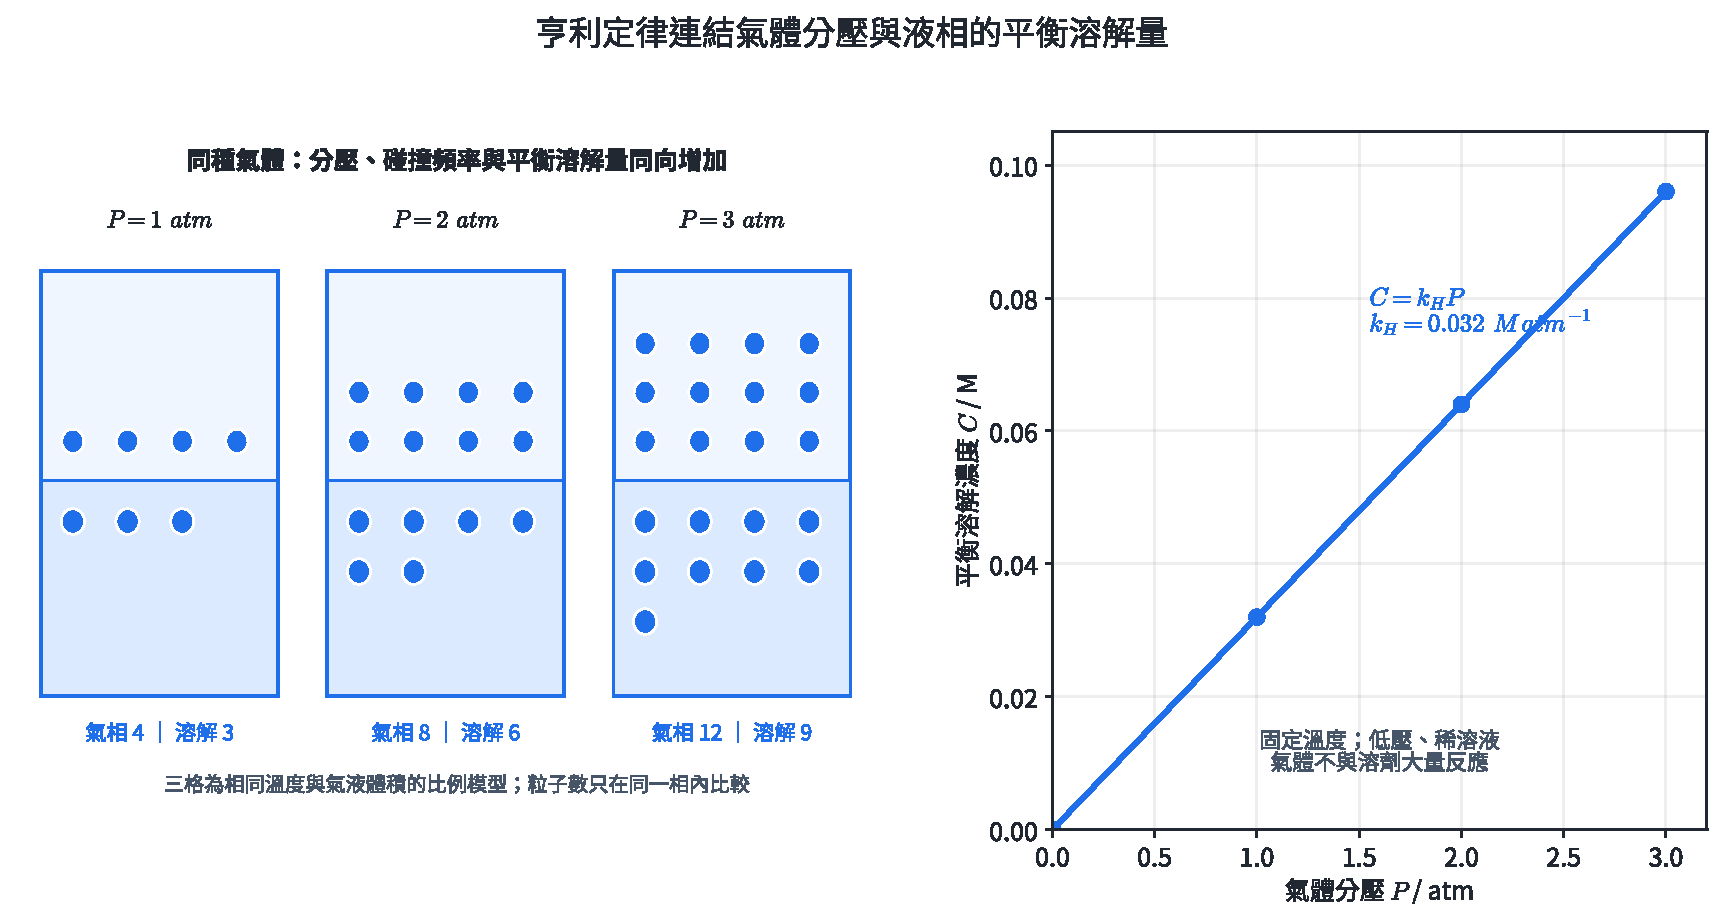
\includegraphics[width=0.98\linewidth,height=\textheight,keepaspectratio,alt={圖 2｜固定溫度與氣液體積時，氣相粒子數及液相平衡溶解粒子數各自在同一相內隨分壓等比增加；兩相使用同一符號表示同一種氣體。}]{assets/選化I-3-亨利定律粒子與數據.pdf}
\caption{圖 2｜固定溫度與氣液體積時，氣相粒子數及液相平衡溶解粒子數各自在同一相內隨分壓等比增加；兩相使用同一符號表示同一種氣體。}
\end{figure}

\begin{HandoutWorkedExample}

\subsection{示範 5｜降壓後的氣體溶解量}\label{ux793aux7bc4-5ux964dux58d3ux5f8cux7684ux6c23ux9ad4ux6eb6ux89e3ux91cf}

\(25^\circ\mathrm C\) 時，某氣體在水中的 \(k_H=0.0320\ \mathrm{mol\,L^{-1}\,atm^{-1}}\)。分壓由 \(0.800\ \mathrm{atm}\) 降至 \(0.250\ \mathrm{atm}\)，求每公升溶液在新平衡前後的溶解量差。

\[
C_i=(0.0320)(0.800)=0.0256\ \mathrm M,
\]

\[
C_f=(0.0320)(0.250)=0.00800\ \mathrm M.
\]

每公升釋出 \(0.0256-0.00800=0.0176\ \mathrm{mol}\)。開啟氣水後 \(CO_2\) 分壓降低而冒泡，潛水上升過快時溶於組織的 \(N_2\) 也可形成氣泡；後者需以減壓程序與實際潛水表管理。

\end{HandoutWorkedExample}

\begin{HandoutWorkedExample}

\subsection{示範 6｜從溶解濃度求混合氣體組成}\label{ux793aux7bc4-6ux5f9eux6eb6ux89e3ux6fc3ux5ea6ux6c42ux6df7ux5408ux6c23ux9ad4ux7d44ux6210}

空氣中氧的莫耳分率為 \(0.210\)，總壓 \(1.00\ \mathrm{atm}\)。某溫度下 \(O_2\) 的 \(k_H=1.30\times10^{-3}\ \mathrm{mol\,L^{-1}\,atm^{-1}}\)。求與空氣平衡的水中 \(O_2\) 濃度。

\[
P_{O_2}=y_{O_2}P_{total}=(0.210)(1.00)=0.210\ \mathrm{atm},
\]

\[
C_{O_2}=(1.30\times10^{-3})(0.210)=2.73\times10^{-4}\ \mathrm{mol\,L^{-1}}.
\]

若水溫上升或水中有耗氧生物與反應，實測溶氧會偏離這個平衡估計；水質監測因此要同時記錄溫度、氣壓與生物狀態。

\end{HandoutWorkedExample}

\subsection{練習 1}\label{ux7df4ux7fd2-1}

\begin{enumerate}
\def\labelenumi{\arabic{enumi}.}
\tightlist
\item
  未知白色固體可能是 \(NaCl\)、砂糖或 \(CaCO_3\)。設計不超過三步的鑑定流程，並寫出每步證據。
\item
  \(12.0\ \mathrm g\) 溶質與 \(188.0\ \mathrm g\) 水形成溶液，求質量百分率。
\item
  飲用水中某金屬離子為 \(2.50\ \mathrm{mg}\)，水樣體積 \(1.25\ \mathrm L\)、密度近似 \(1.00\ \mathrm{kg\,L^{-1}}\)。求 \(\mathrm{mg\,L^{-1}}\) 與 ppm。
\item
  \(0.250\ \mathrm{mol}\) 尿素溶於 \(500\ \mathrm g\) 水，最後配成 \(600\ \mathrm{mL}\) 溶液。求 \(C_m\) 與 \(C_M\)。
\item
  某氣體在 \(20^\circ\mathrm C\) 的 \(k_H=0.0200\ \mathrm{mol\,L^{-1}\,atm^{-1}}\)。分壓由 \(1.50\ \mathrm{atm}\) 降至 \(0.400\ \mathrm{atm}\)時，\(2.00\ \mathrm L\) 溶液最多釋出多少莫耳氣體？
\item
  同溫三次平衡數據如下，判斷哪一次不符合同一個亨利常數，並提出一個可檢驗原因。
\end{enumerate}

{\def\LTcaptype{none} % do not increment counter
\begin{longtable}[]{@{}rrr@{}}
\toprule\noalign{}
實驗 & 分壓 / atm & 平衡濃度 / \(\mathrm{mol\,L^{-1}}\) \\
\midrule\noalign{}
\endhead
\bottomrule\noalign{}
\endlastfoot
I & 0.50 & 0.0100 \\
II & 1.00 & 0.0202 \\
III & 1.50 & 0.0240 \\
\end{longtable}
}

\subsection{練習 1 解析}\label{ux7df4ux7fd2-1-ux89e3ux6790}

\begin{enumerate}
\def\labelenumi{\arabic{enumi}.}
\tightlist
\item
  加水：\(CaCO_3\) 幾乎不溶，\(NaCl\) 與砂糖溶解。對可溶樣品測導電度：\(NaCl\) 溶液顯著導電，砂糖溶液導電度很低。對不溶樣品加稀酸：\(CaCO_3\) 釋出 \(CO_2\)，可再用石灰水確認。
\item
  溶液質量 \(=200.0\ \mathrm g\)，質量百分率 \(=12.0/200.0\times100\%=6.00\%\)。
\item
  \(2.50/1.25=2.00\ \mathrm{mg\,L^{-1}}\)。在題設密度與稀薄條件下約為 \(2.00\ \mathrm{ppm}\)。
\item
  \(C_m=0.250/0.500=0.500\ \mathrm{mol\,kg^{-1}}\)；\(C_M=0.250/0.600=0.417\ \mathrm{mol\,L^{-1}}\)。
\item
  \(\Delta C=(0.0200)(1.50-0.400)=0.0220\ \mathrm{mol\,L^{-1}}\)，釋出量 \(=(0.0220)(2.00)=0.0440\ \mathrm{mol}\)。
\item
  \(C/P\) 分別為 \(0.0200\)、\(0.0202\)、\(0.0160\ \mathrm{mol\,L^{-1}\,atm^{-1}}\)，III 偏離。可檢驗 III 的溫度是否較高、是否未達平衡、氣液漏失，或濃度感測器是否超出線性範圍。
\end{enumerate}

\section{2. 蒸氣壓}\label{ux84b8ux6c23ux58d3}

\subsection{2.1 飽和蒸氣壓、沸點與相對濕度}\label{ux98fdux548cux84b8ux6c23ux58d3ux6cb8ux9edeux8207ux76f8ux5c0dux6fd5ux5ea6}

液體表面的部分粒子具有足夠動能可進入氣相，這個過程是\textbf{蒸發}；氣相粒子返回液相是\textbf{凝結}。密閉容器中若液相仍存在，當蒸發速率與凝結速率相等時建立動態平衡。此時蒸氣的分壓稱為該液體在該溫度的\textbf{飽和蒸氣壓} \(P^*\)。

對純物質，\(P^*\) 主要由溫度與分子間作用力決定。溫度越高，高能粒子比例越大，\(P^*\) 上升；同溫時分子間吸引較強的物質通常 \(P^*\) 較低。只要氣、液兩相仍共存，改變液體量或容器氣相體積會改變達平衡所需的蒸發量，最後 \(P^*\) 由同一溫度決定。

\textbf{沸騰}是液體內部氣泡可穩定生長的汽化；條件為

\[
P^*(T_b)=P_{external}.
\]

降低外壓會使交點移到較低溫，因此高山上的水沸點較低，真空濃縮也能用較低溫移除溶劑。

\begin{figure}
\centering
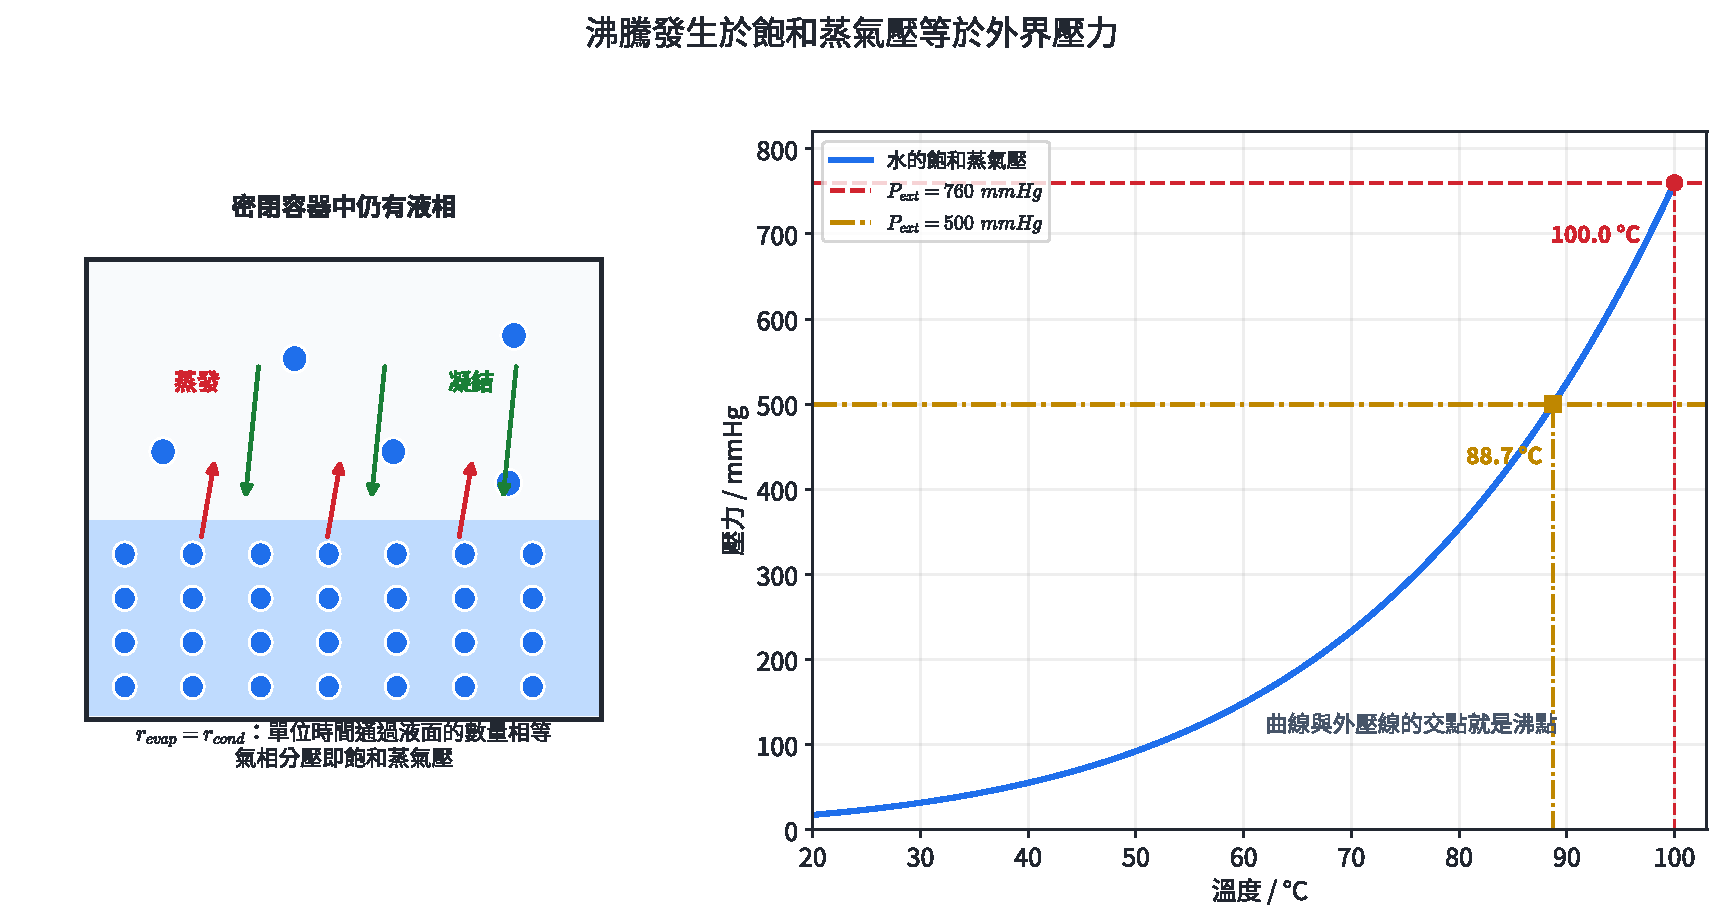
\includegraphics[width=0.98\linewidth,height=\textheight,keepaspectratio,alt={圖 3｜密閉容器中蒸發、凝結速率相等的動態平衡，及水的飽和蒸氣壓曲線與 760、500 mmHg 外壓線的交點。箭頭數只表示相等速率。}]{assets/選化I-3-蒸氣壓與沸點.pdf}
\caption{圖 3｜密閉容器中蒸發、凝結速率相等的動態平衡，及水的飽和蒸氣壓曲線與 760、500 mmHg 外壓線的交點。箭頭數只表示相等速率。}
\end{figure}

\begin{HandoutWorkedExample}

\subsection{示範 7｜由蒸氣壓資料求沸點}\label{ux793aux7bc4-7ux7531ux84b8ux6c23ux58d3ux8cc7ux6599ux6c42ux6cb8ux9ede}

某地大氣壓為 \(500\ \mathrm{mmHg}\)。由圖 3 的水蒸氣壓曲線估計沸點，並比較此地與 \(760\ \mathrm{mmHg}\) 下煮食的差異。

曲線上 \(P^*=500\ \mathrm{mmHg}\) 的交點約 \(88.7^\circ\mathrm C\)；\(760\ \mathrm{mmHg}\) 的交點約 \(100.0^\circ\mathrm C\)。前者的沸水溫度較低，需要較長加熱時間才能達到同程度的食材軟化或蛋白質變性。

\end{HandoutWorkedExample}

\textbf{相對濕度} \(RH\) 比較空氣中實際水蒸氣分壓 \(P_{H_2O}\) 與同溫飽和水蒸氣壓 \(P_{H_2O}^*(T)\)：

\[
RH=\frac{P_{H_2O}}{P_{H_2O}^*(T)}\times100\%.
\]

保持實際水氣量而升溫時，分母上升，\(RH\) 下降。空氣冷卻到飽和時的溫度稱為\textbf{露點}；繼續冷卻時，部分水氣凝結，直到氣相分壓等於新溫度的飽和壓。

\begin{figure}
\centering
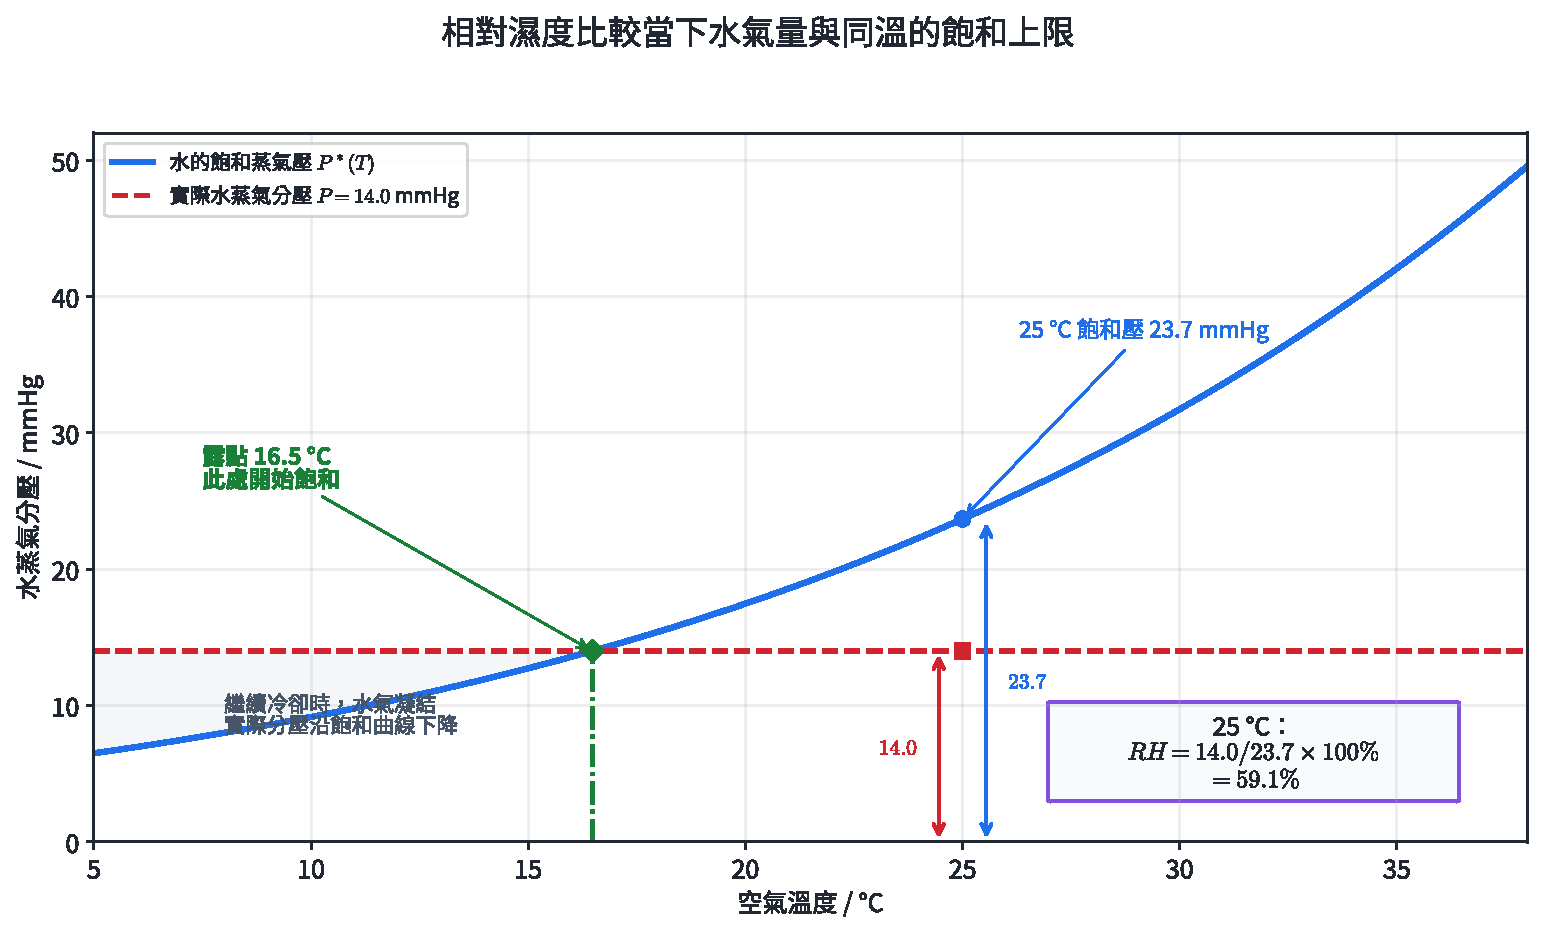
\includegraphics[width=0.92\linewidth,height=\textheight,keepaspectratio,alt={圖 4｜25 °C 時，共用零點的 14.0 與 23.7 mmHg 兩個壓力高度之比給出相對濕度；14.0 mmHg 橫線與飽和曲線交於 16.5 °C，即露點。}]{assets/選化I-3-相對濕度與露點.pdf}
\caption{圖 4｜25 °C 時，共用零點的 14.0 與 23.7 mmHg 兩個壓力高度之比給出相對濕度；14.0 mmHg 橫線與飽和曲線交於 16.5 °C，即露點。}
\end{figure}

\begin{HandoutWorkedExample}

\subsection{示範 8｜相對濕度與露點}\label{ux793aux7bc4-8ux76f8ux5c0dux6fd5ux5ea6ux8207ux9732ux9ede}

\(25.0^\circ\mathrm C\) 時水的飽和蒸氣壓為 \(23.7\ \mathrm{mmHg}\)，空氣中實際水氣分壓為 \(14.0\ \mathrm{mmHg}\)。求相對濕度，並由圖 4 估計露點。

\[
RH=\frac{14.0}{23.7}\times100\%=59.1\%.
\]

在飽和曲線上尋找 \(P^*=14.0\ \mathrm{mmHg}\)，得露點約 \(16.5^\circ\mathrm C\)。冷氣出風口、窗面與電子設備若低於露點，表面可能結露；濕度控制要同時考慮水氣量與表面溫度。

\end{HandoutWorkedExample}

\subsection{2.2 拉午耳定律與氣相組成}\label{ux62c9ux5348ux8033ux5b9aux5f8bux8207ux6c23ux76f8ux7d44ux6210}

對理想溶液，成分 \(i\) 的平衡分壓為

\[
P_i=X_iP_i^*,
\]

其中 \(X_i\) 是該成分在液相的莫耳分率，\(P_i^*\) 是純成分在同溫的飽和蒸氣壓。各分壓相加得總壓：

\[
P_{total}=\sum_iP_i.
\]

若溶質 \(B\) 難揮發，\(P_B\approx0\)，則

\[
P_{solution}=X_AP_A^*,\qquad
\Delta P=X_BP_A^*,\qquad
\frac{\Delta P}{P_A^*}=X_B.
\]

這是難揮發、非電解溶質在理想稀溶液中的依數性關係：大小由溶質粒子數決定。若 A、B 都可揮發，氣相莫耳分率由

\[
y_A=\frac{P_A}{P_{total}}
\]

求得。蒸氣相會富含 \(P_i^*\) 較大、較易揮發的成分，這是蒸餾分離的核心。

\begin{figure}
\centering
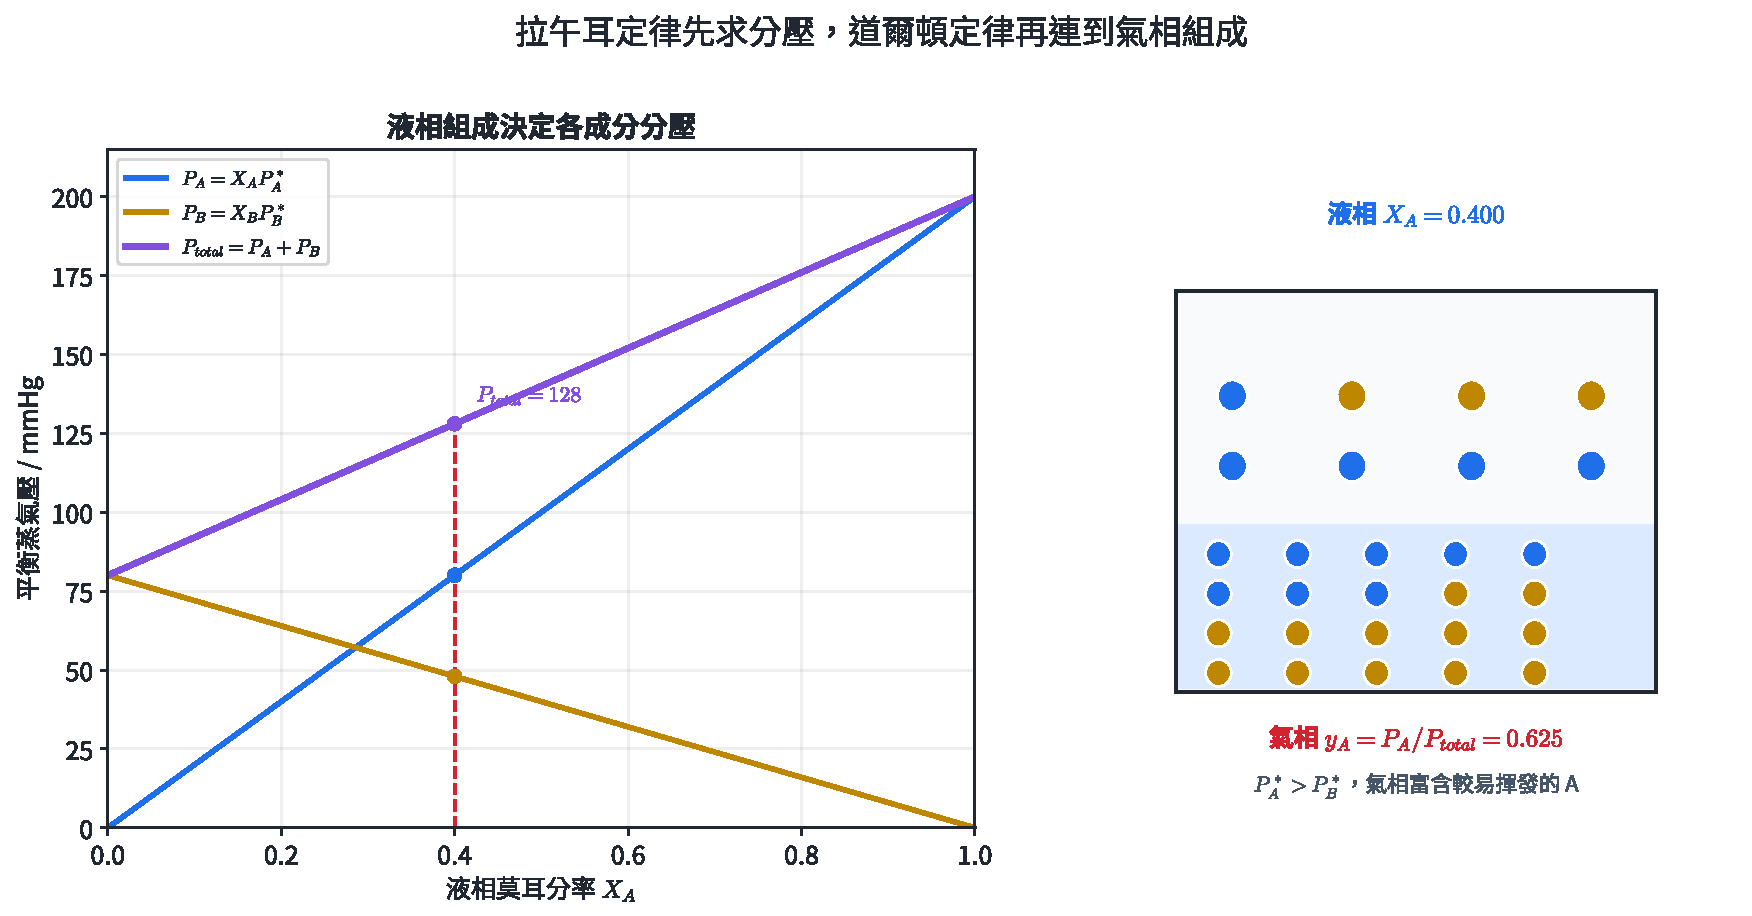
\includegraphics[width=0.98\linewidth,height=\textheight,keepaspectratio,alt={圖 5｜二元理想溶液中的分壓、總壓與氣相組成；在 X\_A=0.400 時，A 因純物質蒸氣壓較大而在氣相富集。}]{assets/選化I-3-拉午耳定律與氣相組成.pdf}
\caption{圖 5｜二元理想溶液中的分壓、總壓與氣相組成；在 \(X_A=0.400\) 時，A 因純物質蒸氣壓較大而在氣相富集。}
\end{figure}

\begin{HandoutWorkedExample}

\subsection{示範 9｜難揮發性溶質的蒸氣壓下降}\label{ux793aux7bc4-9ux96e3ux63eeux767cux6027ux6eb6ux8ceaux7684ux84b8ux6c23ux58d3ux4e0bux964d}

將 \(2.00\ \mathrm{mol}\) 葡萄糖溶於 \(18.0\ \mathrm{mol}\) 水。某溫度下純水蒸氣壓為 \(24.0\ \mathrm{mmHg}\)，求理想溶液的水蒸氣壓與下降量。

\[
X_{H_2O}=\frac{18.0}{20.0}=0.900,
\]

\[
P_{H_2O}=(0.900)(24.0)=21.6\ \mathrm{mmHg},\qquad
\Delta P=2.40\ \mathrm{mmHg}.
\]

也可用 \(X_{solute}=0.100\) 直接得 \(\Delta P=(0.100)(24.0)\)。

\end{HandoutWorkedExample}

\begin{HandoutWorkedExample}

\subsection{示範 10｜可揮發二元溶液的氣相組成}\label{ux793aux7bc4-10ux53efux63eeux767cux4e8cux5143ux6eb6ux6db2ux7684ux6c23ux76f8ux7d44ux6210}

在某溫度，\(P_A^*=200\ \mathrm{mmHg}\)、\(P_B^*=80.0\ \mathrm{mmHg}\)，理想溶液的 \(X_A=0.400\)。

\[
P_A=(0.400)(200)=80.0\ \mathrm{mmHg},
\]

\[
P_B=(0.600)(80.0)=48.0\ \mathrm{mmHg}.
\]

\[
P_{total}=128\ \mathrm{mmHg},\qquad y_A=\frac{80.0}{128}=0.625.
\]

\(y_A>X_A\)，氣相比液相更富含 A。收集氣相凝結物可讓館出物中 A 的比例上升。

\end{HandoutWorkedExample}

\subsection{2.3 理想、非理想與密閉容器的質量轉移}\label{ux7406ux60f3ux975eux7406ux60f3ux8207ux5bc6ux9589ux5bb9ux5668ux7684ux8ceaux91cfux8f49ux79fb}

理想溶液在全組成範圍近似遵守拉午耳定律，通常意味著 A--B 作用力與 A--A、B--B 作用力的平均相近，混合體積變化與混合熱都很小。

\begin{itemize}
\tightlist
\item
  \textbf{正偏差}：實測蒸氣壓高於理想值。A--B 吸引較弱，粒子較易離開液相；常伴隨 \(\Delta H_{mix}>0\)、\(\Delta V_{mix}>0\)。
\item
  \textbf{負偏差}：實測蒸氣壓低於理想值。A--B 吸引較強，粒子較難離開液相；常伴隨 \(\Delta H_{mix}<0\)、\(\Delta V_{mix}<0\)。
\end{itemize}

高濃度、強氫鍵、離子--偶極作用或明顯結構差異都可使理想近似變差。

\begin{figure}
\centering
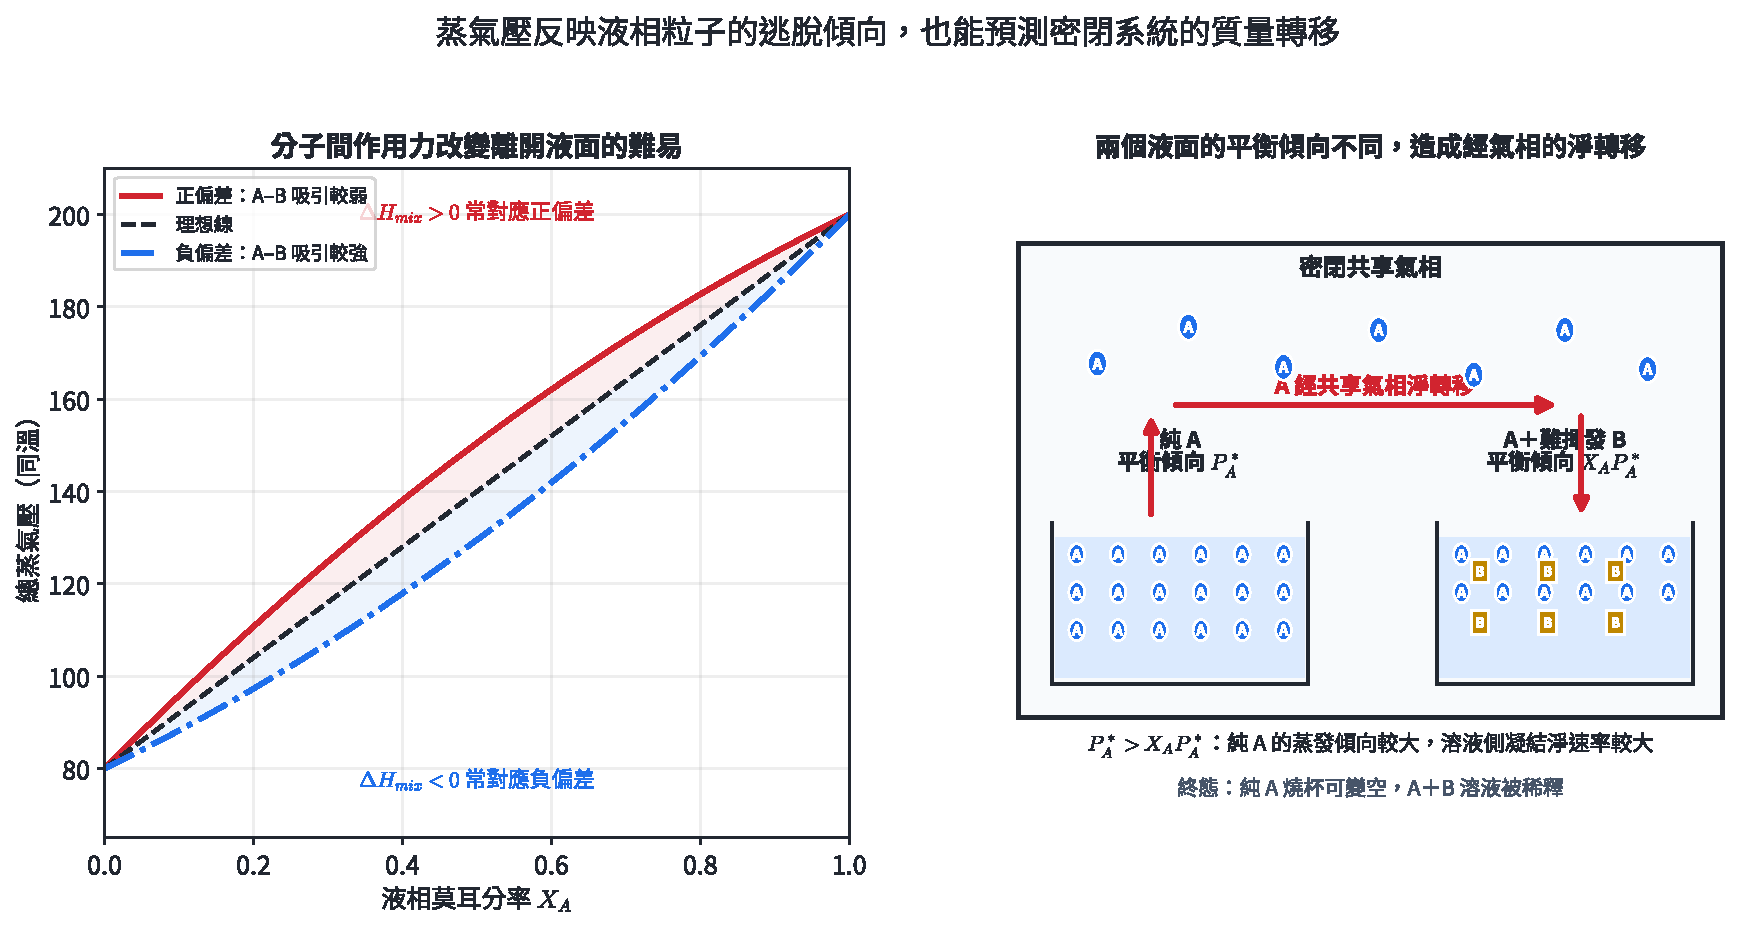
\includegraphics[width=0.98\linewidth,height=\textheight,keepaspectratio,alt={圖 6｜非理想溶液的正、負蒸氣壓偏差；同一密閉氣相中，純溶劑與溶液液面的平衡傾向不同，使溶劑經氣相淨轉移到溶液側。}]{assets/選化I-3-非理想偏差與密閉轉移.pdf}
\caption{圖 6｜非理想溶液的正、負蒸氣壓偏差；同一密閉氣相中，純溶劑與溶液液面的平衡傾向不同，使溶劑經氣相淨轉移到溶液側。}
\end{figure}

同一密閉容器中，一杯純溶劑與一杯含難揮發性溶質的溶液共享氣相。純溶劑平衡蒸氣壓較大，溶劑經氣相淨轉移至溶液側。兩側均持續蒸發與凝結，淨速率由兩個液面的逃脫傾向差決定。在沒有溢流與其他相轉的封閉模型中，純溶劑杯最後耗盡，稀釋後的溶液再與氣相建立新平衡。

\begin{HandoutWorkedExample}

\subsection{示範 11｜用蒸氣壓偏差判斷粒子間作用力}\label{ux793aux7bc4-11ux7528ux84b8ux6c23ux58d3ux504fux5deeux5224ux65b7ux7c92ux5b50ux9593ux4f5cux7528ux529b}

某 \(X_A=0.50\) 的二元溶液，理想總蒸氣壓為 \(140\ \mathrm{mmHg}\)，實測值為 \(158\ \mathrm{mmHg}\)，絕熱混合時溫度降低。

\(158>140\)，故為正偏差，顯示 A--B 平均吸引弱於原有作用力。混合時溶液本身降溫，表示它從周圍吸熱，\(\Delta H_{mix}>0\)。兩項證據相互支持。

\end{HandoutWorkedExample}

\begin{HandoutWorkedExample}

\subsection{示範 12｜密閉容器中的溶劑轉移}\label{ux793aux7bc4-12ux5bc6ux9589ux5bb9ux5668ux4e2dux7684ux6eb6ux5291ux8f49ux79fb}

密閉容器中放兩個開口小杯：甲盛純水，乙盛葡萄糖水溶液。溫度固定，葡萄糖難揮發。甲杯液面上的平衡水蒸氣壓為 \(P_{H_2O}^*\)，乙杯約為 \(X_{H_2O}P_{H_2O}^*\)，後者較小。初期淨效果是水由甲杯經蒸氣轉移至乙杯。乙杯的水增加、葡萄糖莫耳數不變，故葡萄糖莫耳分率與重量莫耳濃度均下降。

\end{HandoutWorkedExample}

\subsection{練習 2}\label{ux7df4ux7fd2-2}

\begin{enumerate}
\def\labelenumi{\arabic{enumi}.}
\tightlist
\item
  在 \(25^\circ\mathrm C\) 且液態水仍存在時，密閉容器體積增為兩倍。說明最終飽和蒸氣壓與達平衡前額外蒸發量如何變化。
\item
  某地外壓 \(600\ \mathrm{mmHg}\)。水的資料為 \(90^\circ\mathrm C:526\ \mathrm{mmHg}\)、\(95^\circ\mathrm C:634\ \mathrm{mmHg}\)。以線性內插估計沸點。
\item
  \(30^\circ\mathrm C\) 的飽和水蒸氣壓為 \(31.8\ \mathrm{mmHg}\)，實際水氣分壓 \(19.1\ \mathrm{mmHg}\)。求 \(RH\)。
\item
  \(1.00\ \mathrm{mol}\) 難揮發性非電解質與 \(9.00\ \mathrm{mol}\) 水形成理想溶液。純水蒸氣壓 \(20.0\ \mathrm{mmHg}\)，求溶液蒸氣壓與相對下降量。
\item
  某理想二元溶液的 \(P_A^*=150\ \mathrm{mmHg}\)、\(P_B^*=50.0\ \mathrm{mmHg}\)，\(X_A=0.300\)。求 \(P_A\)、\(P_B\)、\(P_{total}\) 與 \(y_A\)。
\item
  三種 \(X_A=0.50\) 混合物的理想總壓均為 \(100\ \mathrm{kPa}\)。I 實測 \(116\ \mathrm{kPa}\) 且絕熱混合後降溫；II 實測 \(84\ \mathrm{kPa}\) 且升溫；III 實測 \(116\ \mathrm{kPa}\) 且升溫。判斷各組偏差，並評估壓力與熱證據是否一致。
\end{enumerate}

\subsection{練習 2 解析}\label{ux7df4ux7fd2-2-ux89e3ux6790}

\begin{enumerate}
\def\labelenumi{\arabic{enumi}.}
\tightlist
\item
  同溫且兩相共存，最終 \(P^*\) 不變。氣相體積增大後，要有更多水分子進入氣相才能恢復同一分壓，因此額外蒸發量增加。
\item
  \(T=90+(600-526)/(634-526)\times5=93.4^\circ\mathrm C\)。交點位於已知資料之間，線性內插可作近似。
\item
  \(RH=19.1/31.8\times100\%=60.1\%\)。
\item
  \(X_{H_2O}=0.900\)，\(P=18.0\ \mathrm{mmHg}\)；\(\Delta P/P^*=X_{solute}=0.100\)，相對下降 \(10.0\%\)。
\item
  \(X_B=0.700\)。\(P_A=45.0\ \mathrm{mmHg}\)，\(P_B=35.0\ \mathrm{mmHg}\)，\(P_{total}=80.0\ \mathrm{mmHg}\)，\(y_A=0.5625\)。
\item
  I 總壓高於理想值，為正偏差；降溫支持 \(\Delta H_{mix}>0\)，一致。II 是負偏差，升溫支持 \(\Delta H_{mix}<0\)，一致。III 的壓力指向正偏差，升溫卻指向放熱，兩項證據不一致；需重複溫度量測、控制熱損失，並確認是否發生反應。
\end{enumerate}

\section{3. 溶液的沸點、凝固點與滲透壓}\label{ux6eb6ux6db2ux7684ux6cb8ux9edeux51ddux56faux9edeux8207ux6ef2ux900fux58d3}

\subsection{3.1 沸點上升與凝固點下降}\label{ux6cb8ux9edeux4e0aux5347ux8207ux51ddux56faux9edeux4e0bux964d}

難揮發性溶質使溶劑莫耳分率小於 1，同溫下溶液的溶劑蒸氣壓低於純溶劑。要使溶液蒸氣壓達外壓，需升到更高溫，因此沸點上升。凝固時，結晶主要排列成純溶劑固體；溶質降低液相溶劑的化學勢，要降到更低溫才能與固相平衡，因此凝固點下降。

\begin{figure}
\centering
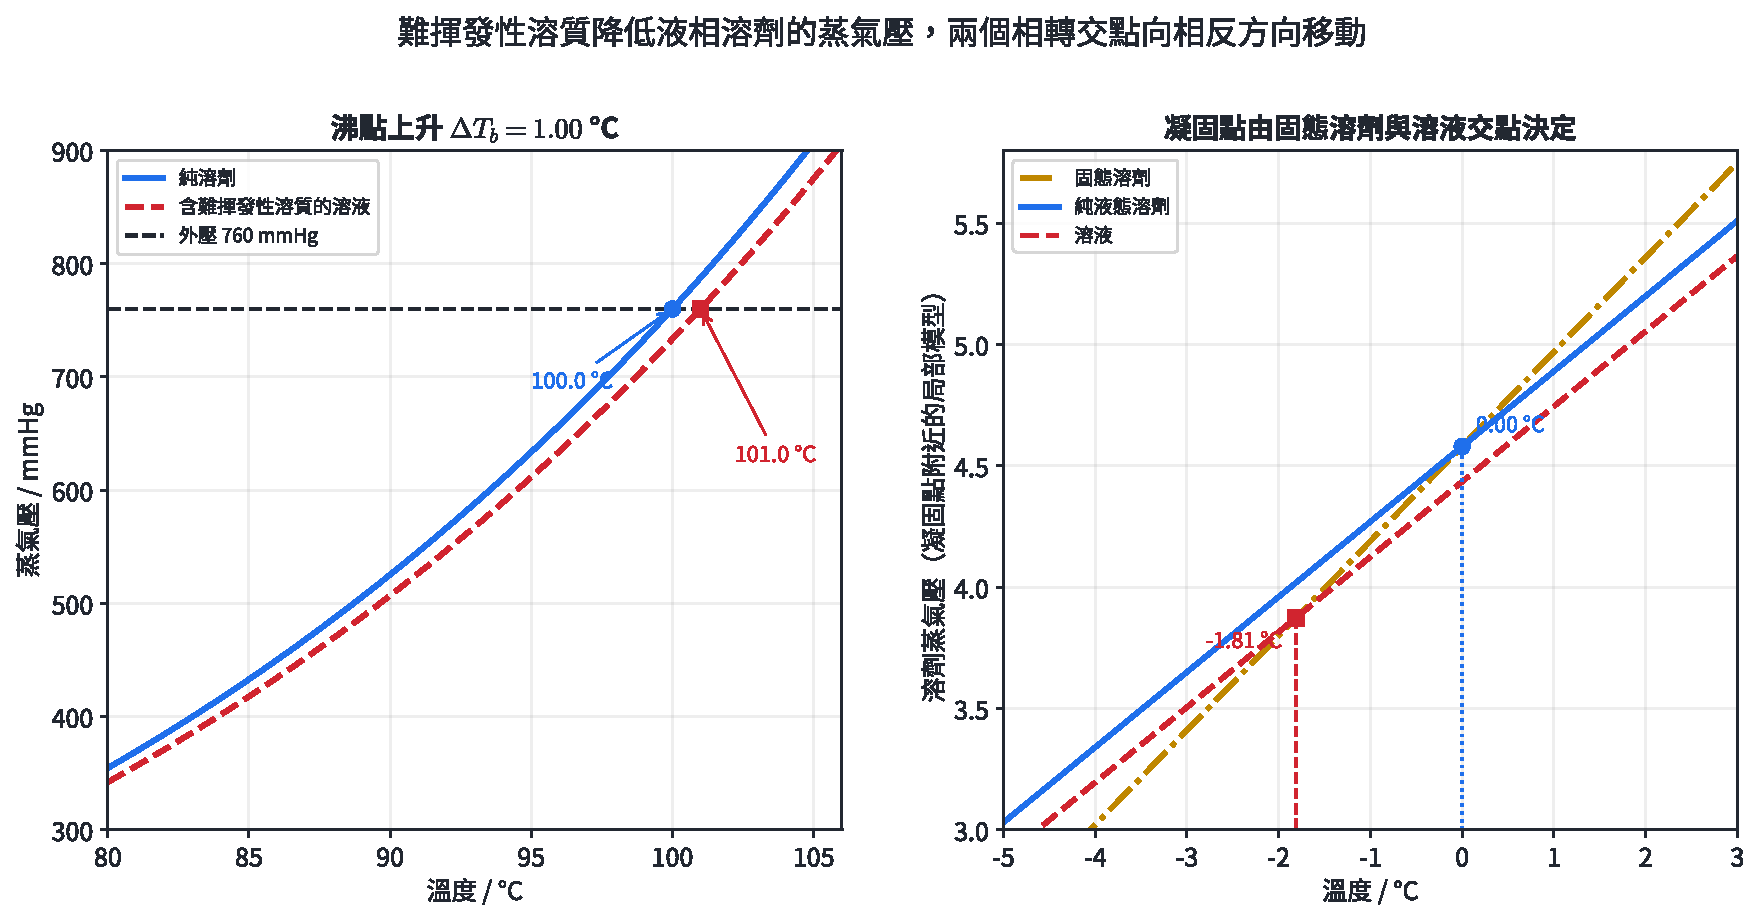
\includegraphics[width=0.98\linewidth,height=\textheight,keepaspectratio,alt={圖 7｜難揮發性溶質降低液相溶劑蒸氣壓：與外壓的沸騰交點移向高溫，與固態溶劑的凝固交點移向低溫。右圖是凝固點附近的局部線性模型。}]{assets/選化I-3-氣壓下降與相轉交點.pdf}
\caption{圖 7｜難揮發性溶質降低液相溶劑蒸氣壓：與外壓的沸騰交點移向高溫，與固態溶劑的凝固交點移向低溫。右圖是凝固點附近的局部線性模型。}
\end{figure}

對稀薄、理想、難揮發、非電解質溶液，

\[
\Delta T_b=T_b(\text{溶液})-T_b^*=K_bC_m,
\]

\[
\Delta T_f=T_f^*-T_f(\text{溶液})=K_fC_m.
\]

\(K_b\)、\(K_f\) 只由溶劑與壓力條件決定，常用單位為 \(\mathrm{K\,kg\,mol^{-1}}\)。溫差的 K 與 \(^\circ\mathrm C\) 數值相同。公式中的 \(C_m\) 直接以每公斤溶劑的溶質莫耳數代入，且少受溫度引起的體積變化影響。

\begin{HandoutWorkedExample}

\subsection{示範 13｜由重量莫耳濃度求沸點與凝固點}\label{ux793aux7bc4-13ux7531ux91cdux91cfux83abux8033ux6fc3ux5ea6ux6c42ux6cb8ux9edeux8207ux51ddux56faux9ede}

\(0.500\ \mathrm m\) 葡萄糖水溶液在 \(1\ \mathrm{atm}\) 下，取水的 \(K_b=0.512\ \mathrm{K\,kg\,mol^{-1}}\)、\(K_f=1.86\ \mathrm{K\,kg\,mol^{-1}}\)，求沸點與凝固點。

\[
\Delta T_b=(0.512)(0.500)=0.256^\circ\mathrm C,
\]

\[
T_b=100.000+0.256=100.256^\circ\mathrm C.
\]

\[
\Delta T_f=(1.86)(0.500)=0.930^\circ\mathrm C,
\]

\[
T_f=0.000-0.930=-0.930^\circ\mathrm C.
\]

兩個溫差都是正的大小；最後用「沸點加、凝固點減」放回溫度軸。

\end{HandoutWorkedExample}

\begin{HandoutWorkedExample}

\subsection{示範 14｜由凝固點下降求莫耳質量}\label{ux793aux7bc4-14ux7531ux51ddux56faux9edeux4e0bux964dux6c42ux83abux8033ux8ceaux91cf}

將 \(3.10\ \mathrm g\) 難揮發性非電解質溶於 \(100.0\ \mathrm g\) 苯，凝固點降低 \(1.28^\circ\mathrm C\)。取苯的 \(K_f=5.12\ \mathrm{K\,kg\,mol^{-1}}\)，求溶質莫耳質量。

\[
C_m=\frac{\Delta T_f}{K_f}=\frac{1.28}{5.12}=0.250\ \mathrm{mol\,kg^{-1}}.
\]

溶劑為 \(0.1000\ \mathrm{kg}\)，故

\[
n_{solute}=(0.250)(0.1000)=0.0250\ \mathrm{mol}.
\]

\[
M=\frac{3.10}{0.0250}=124\ \mathrm{g\,mol^{-1}}.
\]

此法測到的是「溶液中獨立粒子」對應的表觀莫耳質量。若溶質解離或聚合，要再納入第 4 節的 \(i\)。

\end{HandoutWorkedExample}

\subsection{3.2 凝固點下降實驗：裝置、證據與誤差}\label{ux51ddux56faux9edeux4e0bux964dux5be6ux9a57ux88ddux7f6eux8b49ux64daux8207ux8aa4ux5dee}

實驗以相同裝置分別測純水與尿素水溶液的冷卻曲線。冰--食鹽混合物提供低於 \(0^\circ\mathrm C\) 的冷浴，小試管與冷浴之間可用大試管留下空氣層，使降溫速率足以記錄。溫度探針測量液體中央，攪拌使內部溫度均勻。

\begin{figure}
\centering
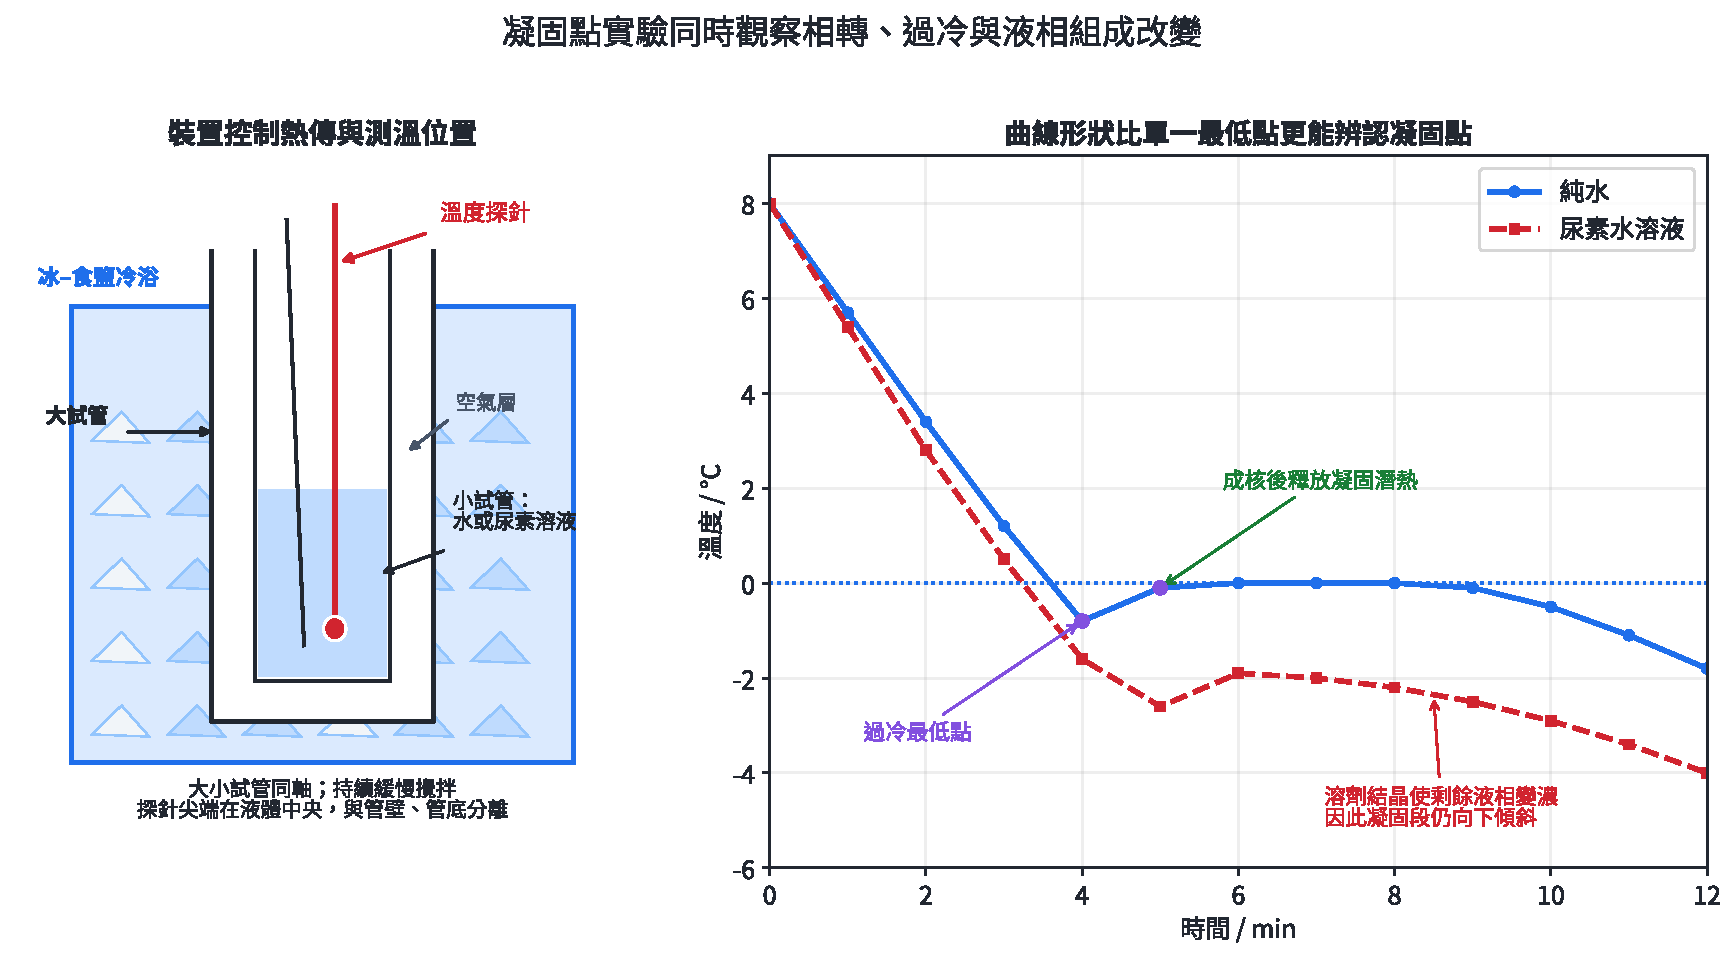
\includegraphics[width=0.98\linewidth,height=\textheight,keepaspectratio,alt={圖 8｜凝固點實驗以小試管同軸置於大試管中，空氣層減緩熱傳；探針尖端位於攪拌中的液體中央。純水有過冷後回升與平臺，溶液在結冰段仍持續降溫。}]{assets/選化I-3-凝固點實驗與冷卻曲線.pdf}
\caption{圖 8｜凝固點實驗以小試管同軸置於大試管中，空氣層減緩熱傳；探針尖端位於攪拌中的液體中央。純水有過冷後回升與平臺，溶液在結冰段仍持續降溫。}
\end{figure}

\textbf{安全與廢棄物}

\begin{itemize}
\tightlist
\item
  配戴護目鏡、實驗衣與適當手套。冰--食鹽浴可造成低溫傷害，以工具移動冰鹽混合物，清理時等待回溫。
\item
  玻璃試管、溫度計與探針要固定，從攪拌與夾持點施力。破裂玻璃放入專用容器。
\item
  尿素及其溶液避免食入、皮膚長時間接觸與粉塵吸入。尿素溶液收集為實驗室指定的含氮水相廢液；冰鹽冷浴依實驗室本地規範排放。
\item
  若做水與乙醇的混合體積、溫度演示，乙醇易燃；工作區無火焰與火花，保持通風，乙醇廢液收入有機溶劑廢液桶。
\end{itemize}

\textbf{觀察--推論}

{\def\LTcaptype{none} % do not increment counter
\begin{longtable}[]{@{}
  >{\raggedright\arraybackslash}p{(\linewidth - 2\tabcolsep) * \real{0.5000}}
  >{\raggedright\arraybackslash}p{(\linewidth - 2\tabcolsep) * \real{0.5000}}@{}}
\toprule\noalign{}
\begin{minipage}[b]{\linewidth}\raggedright
觀察
\end{minipage} & \begin{minipage}[b]{\linewidth}\raggedright
可由資料支持的推論
\end{minipage} \\
\midrule\noalign{}
\endhead
\bottomrule\noalign{}
\endlastfoot
純水先降到 \(0^\circ\mathrm C\) 以下，後回升 & 水曾過冷；成核後凝固潛熱使溫度回升 \\
純水凝固期間出現近水平段 & 固、液兩相共存時，組成近似不變，移除的熱主要用於相轉 \\
尿素溶液開始結冰的溫度較低 & 溶質使溶劑凝固點下降 \\
溶液結冰段仍向下傾斜 & 溶劑結晶後，剩餘液相的尿素濃度上升，其凝固點持續下降 \\
\end{longtable}
}

\begin{HandoutWorkedExample}

\subsection{示範 15｜從冷卻曲線選取凝固點}\label{ux793aux7bc4-15ux5f9eux51b7ux537bux66f2ux7ddaux9078ux53d6ux51ddux56faux9ede}

某純溶劑冷卻資料依序為 \(3.0\)、\(1.2\)、\(-0.7\)、\(0.1\)、\(0.0\)、\(0.0\)、\(-0.1^\circ\mathrm C\)。何者代表過冷最低點？凝固點如何估計？

\(-0.7^\circ\mathrm C\) 是成核前的過冷最低點，不代表平衡凝固點。結晶後釋放潛熱，溫度回到約 \(0.0^\circ\mathrm C\) 的平臺，故凝固點估為 \(0.0^\circ\mathrm C\)。對無平臺的溶液，可以凝固前降溫線與開始結晶後趨勢線的交點作一致估計。

\end{HandoutWorkedExample}

\begin{HandoutWorkedExample}

\subsection{示範 16｜由實驗溫差回求溶質量}\label{ux793aux7bc4-16ux7531ux5be6ux9a57ux6eabux5deeux56deux6c42ux6eb6ux8ceaux91cf}

以 \(50.0\ \mathrm g\) 水配製尿素溶液，測得 \(\Delta T_f=1.24^\circ\mathrm C\)。取 \(K_f(\mathrm{H_2O})=1.86\ \mathrm{K\,kg\,mol^{-1}}\)、\(M(\text{尿素})=60.0\ \mathrm{g\,mol^{-1}}\)，假設理想，求尿素質量。

\[
C_m=\frac{1.24}{1.86}=0.667\ \mathrm{mol\,kg^{-1}}.
\]

\[
n=(0.667)(0.0500)=0.0333\ \mathrm{mol},
\]

\[
m=(0.0333)(60.0)=2.00\ \mathrm g.
\]

若探針貼管壁而讀到過低溫度，\(\Delta T_f\) 會偏大，回算的濃度與尿素量也偏大。

\end{HandoutWorkedExample}

\textbf{主要誤差與改進}

{\def\LTcaptype{none} % do not increment counter
\begin{longtable}[]{@{}
  >{\raggedright\arraybackslash}p{(\linewidth - 4\tabcolsep) * \real{0.3333}}
  >{\raggedright\arraybackslash}p{(\linewidth - 4\tabcolsep) * \real{0.3333}}
  >{\raggedright\arraybackslash}p{(\linewidth - 4\tabcolsep) * \real{0.3333}}@{}}
\toprule\noalign{}
\begin{minipage}[b]{\linewidth}\raggedright
來源
\end{minipage} & \begin{minipage}[b]{\linewidth}\raggedright
對曲線的影響
\end{minipage} & \begin{minipage}[b]{\linewidth}\raggedright
改進
\end{minipage} \\
\midrule\noalign{}
\endhead
\bottomrule\noalign{}
\endlastfoot
探針觸及管壁或管底 & 容易讀到較低的局部溫度 & 固定探針在液體中央，每組深度一致 \\
攪拌不均 & 樣品內有溫度梯度，資料抖動 & 以相同速率連續緩慢攪拌 \\
冷浴溫度或接觸面積不同 & 降溫速率失去可比性 & 使用同一種冷浴配比、浸沒深度與試管 \\
過冷與成核時間隨機 & 最低點變化大 & 以平臺或兩趨勢線交點判讀，並重複實驗 \\
稱量、水分蒸發或樣品殘留 & 實際 \(C_m\) 偏離配方 & 密閉秤量、完全轉移，實驗前後做質量帳 \\
\end{longtable}
}

\subsection{3.3 滲透壓與逆滲透}\label{ux6ef2ux900fux58d3ux8207ux9006ux6ef2ux900f}

\textbf{半透膜}允許溶劑通過，但對題目中的溶質具有足夠截留性。當半透膜兩側溶劑相同、溶質粒子濃度不同時，溶劑由較低溶質粒子濃度側淨流向較高側，此過程為\textbf{滲透}。要恰好阻止此淨流所需施加在溶液側的額外壓力，稱為\textbf{滲透壓} \(\pi\)。

對稀薄、理想、非電解質溶液，

\[
\pi=C_MRT.
\]

溫度要用 K，\(R\) 的單位必須與壓力一致。滲透壓在極稀溶液仍可明顯量測，因此適合求聚合物或大分子的莫耳質量。

\begin{figure}
\centering
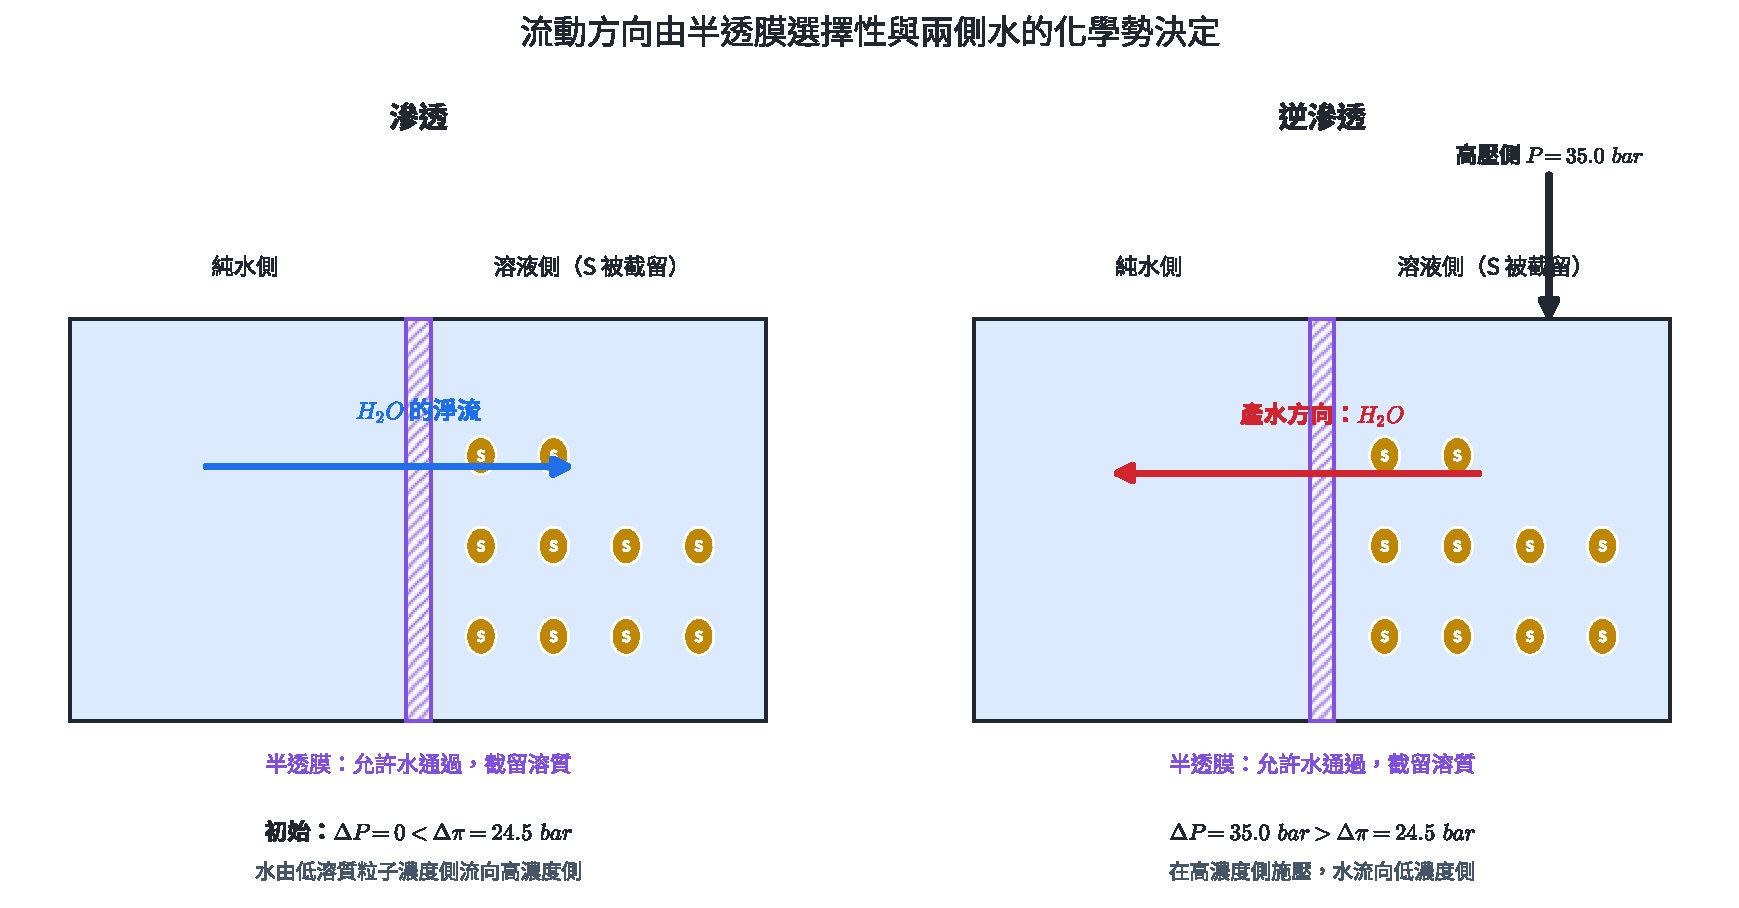
\includegraphics[width=0.98\linewidth,height=\textheight,keepaspectratio,alt={圖 9｜初始壓差小於滲透壓差時，水由純水側流向溶液側；在溶液側施加大於滲透壓差的操作壓差，水的淨流反向，而溶質被膜截留。}]{assets/選化I-3-滲透與逆滲透.pdf}
\caption{圖 9｜初始壓差小於滲透壓差時，水由純水側流向溶液側；在溶液側施加大於滲透壓差的操作壓差，水的淨流反向，而溶質被膜截留。}
\end{figure}

\begin{HandoutWorkedExample}

\subsection{示範 17｜體液溫度的滲透壓}\label{ux793aux7bc4-17ux9ad4ux6db2ux6eabux5ea6ux7684ux6ef2ux900fux58d3}

\(0.150\ \mathrm M\) 葡萄糖水溶液在 \(37.0^\circ\mathrm C\)，假設理想，取 \(R=0.08206\ \mathrm{L\,atm\,mol^{-1}\,K^{-1}}\)，求滲透壓。

\[
T=37.0+273.15=310.15\ \mathrm K,
\]

\[
\pi=(0.150)(0.08206)(310.15)=3.82\ \mathrm{atm}.
\]

醫療輸液的滲透性要與血漿可比，同時考慮溶質是否解離、能否穿過細胞膜，以及真實溶液的非理想性。

\end{HandoutWorkedExample}

\begin{HandoutWorkedExample}

\subsection{示範 18｜由滲透壓求聚合物莫耳質量}\label{ux793aux7bc4-18ux7531ux6ef2ux900fux58d3ux6c42ux805aux5408ux7269ux83abux8033ux8ceaux91cf}

\(2.00\ \mathrm g\) 聚合物配成 \(100.0\ \mathrm{mL}\) 溶液，\(25.0^\circ\mathrm C\) 的滲透壓為 \(0.246\ \mathrm{atm}\)。假設理想，求莫耳質量。

\[
n=\frac{\pi V}{RT}=\frac{(0.246)(0.1000)}{(0.08206)(298.15)}=1.01\times10^{-3}\ \mathrm{mol}.
\]

\[
M=\frac{2.00}{1.01\times10^{-3}}=1.99\times10^3\ \mathrm{g\,mol^{-1}}.
\]

溶液體積必須以 L 代入；若聚合物在溶液中纏合，測得粒子數偏少，回算莫耳質量會偏大。

\end{HandoutWorkedExample}

\textbf{逆滲透}在高濃度側施加 \(P_{applied}>\pi\)，使溶劑逆著自發滲透方向穿過膜。海水淡化、超純水製程與廢水回收都用到這個操作。實際工程壓力需高於熱力學滲透壓，以提供有限通量並克服流道壓降；能耗、膜污染、鹽水濃縮液處理與能量回收也是設計的一部分。

\begin{HandoutWorkedExample}

\subsection{示範 19｜逆滲透的最低熱力條件}\label{ux793aux7bc4-19ux9006ux6ef2ux900fux7684ux6700ux4f4eux71b1ux529bux689dux4ef6}

某鹽水的滲透壓為 \(24.5\ \mathrm{bar}\)，產水側背壓 \(1.0\ \mathrm{bar}\)。判斷在鹽水側施壓 \(20.0\)、\(25.0\)、\(35.0\ \mathrm{bar}\) 時的理想淨流方向。

有效水力壓差為 \(P_{feed}-P_{product}\)。三組分別是 \(19.0\)、\(24.0\)、\(34.0\ \mathrm{bar}\)。前兩者小於 \(24.5\ \mathrm{bar}\)，理想淨流仍指向鹽水側；\(35.0\ \mathrm{bar}\) 時有效差 \(34.0\ \mathrm{bar}>24.5\ \mathrm{bar}\)，可產生逆滲透產水。工程操作還需更高驅動壓差才有可用通量。

\end{HandoutWorkedExample}

\subsection{練習 3}\label{ux7df4ux7fd2-3}

\begin{enumerate}
\def\labelenumi{\arabic{enumi}.}
\tightlist
\item
  \(0.250\ \mathrm m\) 尿素水溶液，取 \(K_b=0.512\)、\(K_f=1.86\ \mathrm{K\,kg\,mol^{-1}}\)，求 \(1\ \mathrm{atm}\) 下沸點與凝固點。
\item
  \(4.00\ \mathrm g\) 難揮發性非電解質溶於 \(80.0\ \mathrm g\) 水，凝固點降低 \(0.775^\circ\mathrm C\)。取 \(K_f=1.86\)，求溶質莫耳質量。
\item
  純水冷卻資料出現 \(0.2\)、\(-1.1\)、\(-0.2\)、\(0.0\)、\(0.0^\circ\mathrm C\)。辨認過冷最低點、凝固點與回溫的能量來源。
\item
  \(0.0750\ \mathrm M\) 葡萄糖溶液在 \(27.0^\circ\mathrm C\) 的滲透壓為何？取 \(R=0.08206\ \mathrm{L\,atm\,mol^{-1}\,K^{-1}}\)。
\item
  \(1.50\ \mathrm g\) 大分子配成 \(250.0\ \mathrm{mL}\) 溶液，\(20.0^\circ\mathrm C\) 測得 \(\pi=0.0144\ \mathrm{atm}\)。求莫耳質量。
\item
  某尿素凝固點實驗的理論 \(\Delta T_f=1.00^\circ\mathrm C\)，三組做法為：I 探針貼管壁；II 緩慢均勻攪拌且重複三次；III 配方後水蒸發一部分。預測 I、III 的測得方向，並說明 II 如何改善證據。
\end{enumerate}

\subsection{練習 3 解析}\label{ux7df4ux7fd2-3-ux89e3ux6790}

\begin{enumerate}
\def\labelenumi{\arabic{enumi}.}
\tightlist
\item
  \(\Delta T_b=(0.512)(0.250)=0.128^\circ\mathrm C\)，\(T_b=100.128^\circ\mathrm C\)。\(\Delta T_f=(1.86)(0.250)=0.465^\circ\mathrm C\)，\(T_f=-0.465^\circ\mathrm C\)。
\item
  \(C_m=0.775/1.86=0.4167\ \mathrm m\)，\(n=(0.4167)(0.0800)=0.0333\ \mathrm{mol}\)，\(M=4.00/0.0333=120\ \mathrm{g\,mol^{-1}}\)。
\item
  \(-1.1^\circ\mathrm C\) 是過冷最低點；成核後回至約 \(0.0^\circ\mathrm C\)，故凝固點約為 \(0.0^\circ\mathrm C\)。回溫的能量來自部分水凝固釋放的潛熱。
\item
  \(T=300.15\ \mathrm K\)，\(\pi=(0.0750)(0.08206)(300.15)=1.85\ \mathrm{atm}\)。
\item
  \(M=mRT/(\pi V)=(1.50)(0.08206)(293.15)/(0.0144\times0.2500)=1.00\times10^4\ \mathrm{g\,mol^{-1}}\)。
\item
  I 可讀到過冷的管壁局部溫度，\(\Delta T_f\) 偏大。III 的溶劑質量減少而 \(C_m\) 上升，\(\Delta T_f\) 偏大。II 減少樣品內溫度梯度，三次重複可估計隨機變異與平均值，使結論不依賴單次成核。
\end{enumerate}

\section{4. 水溶液的依數性}\label{ux6c34ux6eb6ux6db2ux7684ux4f9dux6578ux6027}

\subsection{4.1 有效粒子與凡特何夫因數}\label{ux6709ux6548ux7c92ux5b50ux8207ux51e1ux7279ux4f55ux592bux56e0ux6578}

\textbf{依數性}是稀溶液中主要由溶質粒子數決定，而與粒子化學身分無直接關係的性質。本章包含蒸氣壓下降、沸點上升、凝固點下降與滲透壓。比較「粒子數」之前，要把配方中的化學式單位轉成溶液中獨立運動的有效粒子。

\textbf{凡特何夫因數} \(i\) 定義為

\[
i=\frac{\text{實際有效溶質粒子濃度}}{\text{以配方式量單位計算的溶質濃度}}.
\]

理想極稀溶液中，非電解質 \(i\approx1\)；\(NaCl\rightarrow Na^++Cl^-\) 給 \(i\approx2\)；\(K_2SO_4\rightarrow2K^++SO_4^{2-}\) 給 \(i\approx3\)。實際電解質的測得 \(i\) 常低於完全解離的整數：離子對會減少可近似獨立的粒子，水合與離子間作用則使溶液偏離理想模型。\(i\) 應視為指定濃度與溫度下的有效值。

\begin{figure}
\centering
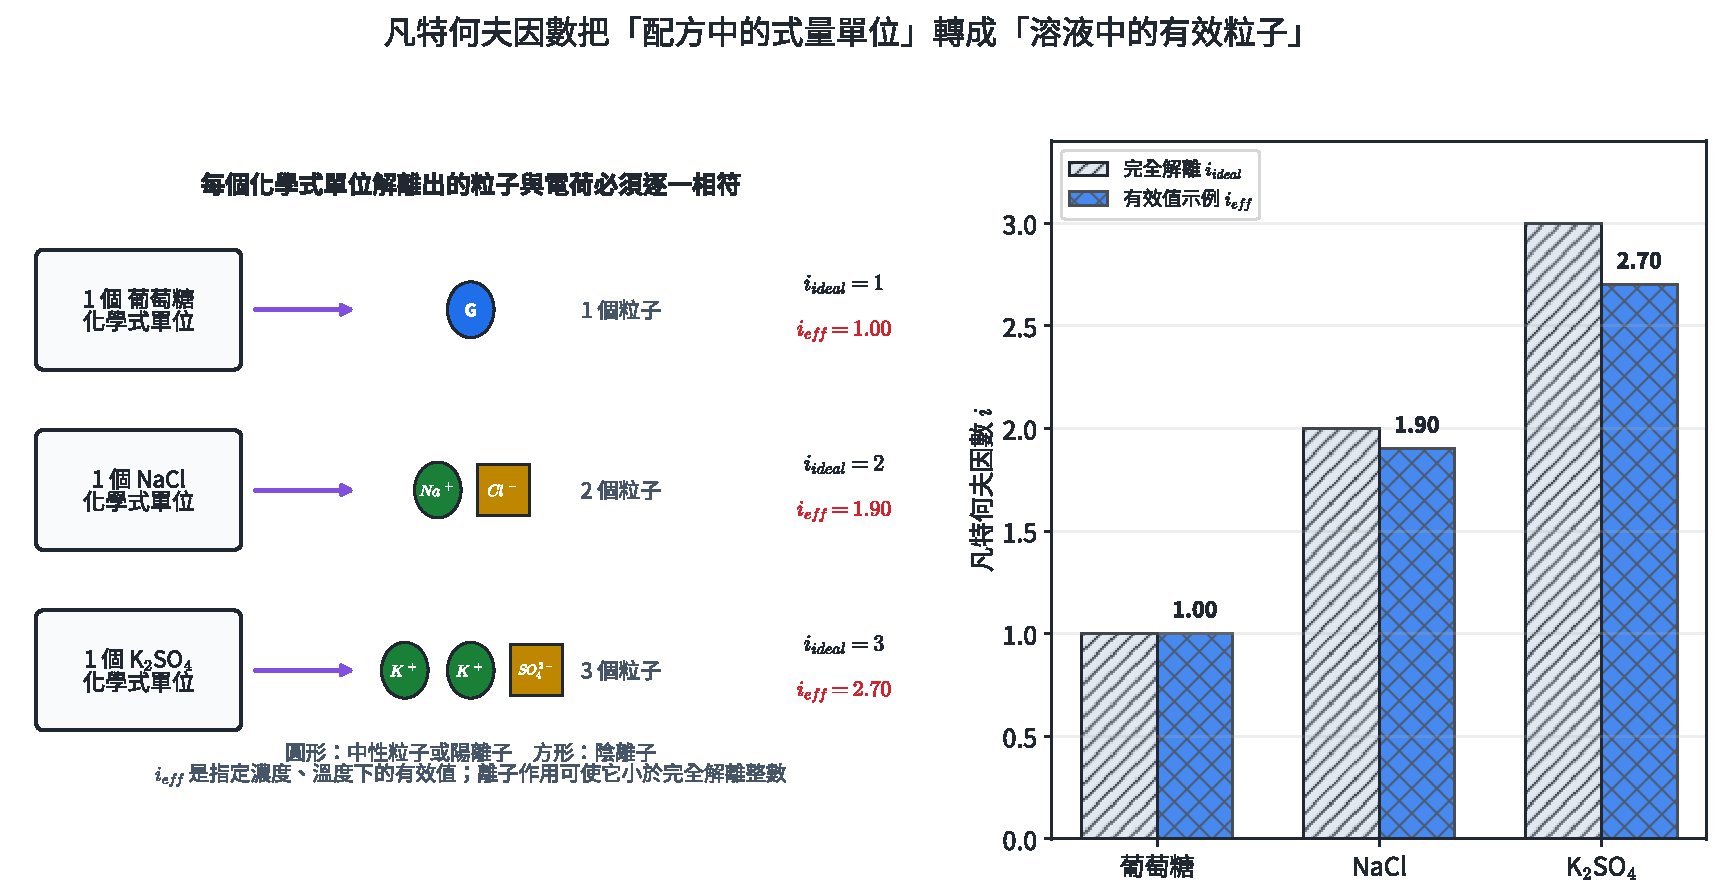
\includegraphics[width=0.98\linewidth,height=\textheight,keepaspectratio,alt={圖 10｜每個葡萄糖、NaCl 與 K\_2SO\_4 化學式單位形成的理論粒子帳；離子數與總電荷逐一守恆。圖中的 i\_\{eff\} 為指定條件下的有效值示例，不是各物質在所有濃度下的固定常數。}]{assets/選化I-3-凡特何夫因數粒子帳.pdf}
\caption{圖 10｜每個葡萄糖、NaCl 與 \(K_2SO_4\) 化學式單位形成的理論粒子帳；離子數與總電荷逐一守恆。圖中的 \(i_{eff}\) 為指定條件下的有效值示例，不是各物質在所有濃度下的固定常數。}
\end{figure}

納入 \(i\) 後，稀溶液公式成為

\[
\frac{\Delta P}{P^*}\approx iX_{formula\ unit},
\]

\[
\Delta T_b=iK_bC_m,\qquad
\Delta T_f=iK_fC_m,\qquad
\pi=iC_MRT.
\]

第一式在非常稀薄時才能用「式量單位莫耳分率×\(i\)」近似實際粒子莫耳分率；若要高精度處理，分母也要改用實際粒子總數。

在偏差主要來自部分解離、且解離後各粒子可近似獨立的簡化模型中，若一個式量單位完全解離可形成 \(\nu\) 個粒子，解離度為 \(\alpha\)，每初始 1 mol 式量單位對應的粒子數為

\[
(1-\alpha)+\nu\alpha=1+\alpha(\nu-1),
\]

因此

\[
i=1+\alpha(\nu-1),\qquad
\alpha=\frac{i-1}{\nu-1}.
\]

\begin{HandoutWorkedExample}

\subsection{示範 20｜由電解質化學式比較依數性}\label{ux793aux7bc4-20ux7531ux96fbux89e3ux8ceaux5316ux5b78ux5f0fux6bd4ux8f03ux4f9dux6578ux6027}

比較同溫、同溶劑、皆為 \(0.100\ \mathrm m\) 的葡萄糖、\(NaCl\)、\(CaCl_2\) 理想極稀溶液之 \(\Delta T_f\)。

葡萄糖不解離，\(i=1\)；\(NaCl\) 形成兩種離子，\(i=2\)；\(CaCl_2\) 形成 \(Ca^{2+}+2Cl^-\)，\(i=3\)。因為 \(K_f\) 與 \(C_m\) 都相同，

\[
\Delta T_f(\text{葡萄糖}):\Delta T_f(NaCl):\Delta T_f(CaCl_2)=1:2:3.
\]

這個整數比是完全解離、理想極稀的上限模型。實測高濃度電解質溶液常偏離這些數值。

\end{HandoutWorkedExample}

\begin{HandoutWorkedExample}

\subsection{\texorpdfstring{示範 21｜由凝固點數據求 \(i\)}{示範 21｜由凝固點數據求 i}}\label{ux793aux7bc4-21ux7531ux51ddux56faux9edeux6578ux64daux6c42-i}

\(0.200\ \mathrm m\) \(NaCl(aq)\) 的凝固點下降為 \(0.707^\circ\mathrm C\)，取 \(K_f(\text{水})=1.86\ \mathrm{K\,kg\,mol^{-1}}\)。求 \(i\)，並與理論值比較。

\[
i=\frac{\Delta T_f}{K_fC_m}=\frac{0.707}{(1.86)(0.200)}=1.90.
\]

完全解離的理論值為 2.00，測得 1.90 表示有效粒子數約為式量單位數的 1.90 倍。若暫時把偏差全歸因於未解離，以簡化模型取 \(\nu=2\)，可定義表觀值

\[
\alpha_{app}=\frac{1.90-1}{2-1}=0.90.
\]

這個 \(\alpha_{app}\) 是依數性模型的表觀參數；\(NaCl\) 的 \(i<2\) 還包含離子間作用等非理想效應，實際解離率需由獨立化學分析判定。

\end{HandoutWorkedExample}

\subsection{4.2 依數性的實用計算與限制}\label{ux4f9dux6578ux6027ux7684ux5be6ux7528ux8a08ux7b97ux8207ux9650ux5236}

依數性可由易測的巨觀數據回推難以直接觀察的粒子數。典型用途包含：

\begin{itemize}
\tightlist
\item
  以 \(\Delta T_f\)、\(\Delta T_b\) 或 \(\pi\) 求未知物莫耳質量。
\item
  以測得 \(i\) 比較電解質的有效粒子數與離子對程度。
\item
  配製防凍液、除冰液、冷凍食品的相轉溫度區間。
\item
  設計醫療等滲透溶液與膜分離製程。
\end{itemize}

公式的共同限制是稀薄與近似理想。濃溶液的粒子間作用、離子水合、溶質纏合或化學反應會使測得值偏離線性關係。海水、體液、高濃度電解質與聚合物溶液的工程計算，會進一步用活性、滲透係數或實測校正。

\begin{HandoutWorkedExample}

\subsection{\texorpdfstring{示範 22｜納入測得 \(i\) 求防凍配方}{示範 22｜納入測得 i 求防凍配方}}\label{ux793aux7bc4-22ux7d0dux5165ux6e2cux5f97-i-ux6c42ux9632ux51cdux914dux65b9}

\(0.750\ \mathrm m\) \(CaCl_2(aq)\) 的測得 \(i=2.60\)，取水 \(K_f=1.86\ \mathrm{K\,kg\,mol^{-1}}\)。求凝固點。

\[
\Delta T_f=(2.60)(1.86)(0.750)=3.63^\circ\mathrm C,
\]

\[
T_f=0.00-3.63=-3.63^\circ\mathrm C.
\]

若直接用完全解離 \(i=3\)，會預測 \(\Delta T_f=4.19^\circ\mathrm C\)，高估防凍效果。真實產品還需由實測凝固曲線、材料腐蝕性與低溫黏度確認可用範圍。

\end{HandoutWorkedExample}

\begin{HandoutWorkedExample}

\subsection{示範 23｜由弱電解質的滲透壓求解離度}\label{ux793aux7bc4-23ux7531ux5f31ux96fbux89e3ux8ceaux7684ux6ef2ux900fux58d3ux6c42ux89e3ux96e2ux5ea6}

\(0.0500\ \mathrm M\) 弱酸 \(HA\) 在 \(25.0^\circ\mathrm C\) 的滲透壓為 \(1.47\ \mathrm{atm}\)，取 \(R=0.08206\ \mathrm{L\,atm\,mol^{-1}\,K^{-1}}\)。\(HA\rightleftharpoons H^++A^-\)，求 \(i\) 與解離度。

\[
i=\frac{\pi}{C_MRT}
=\frac{1.47}{(0.0500)(0.08206)(298.15)}=1.20.
\]

此反應完全解離時 \(\nu=2\)，故

\[
\alpha=\frac{i-1}{2-1}=0.20.
\]

約 \(20\%\) 式量單位解離。題設把溶液視為理想；若濃度較高，活性與膜對離子的截留率都可影響由滲透壓回推的結果。

\end{HandoutWorkedExample}

\subsection{練習 4}\label{ux7df4ux7fd2-4}

\begin{enumerate}
\def\labelenumi{\arabic{enumi}.}
\tightlist
\item
  寫出理想極稀時尿素、\(KCl\)、\(AlCl_3\) 的理論 \(i\)，並比較同 \(C_m\) 水溶液的 \(\Delta T_b\)。
\item
  \(0.300\ \mathrm m\) \(KCl(aq)\) 的 \(\Delta T_f=1.03^\circ\mathrm C\)，取 \(K_f=1.86\)，求 \(i\)。
\item
  某 \(AB_2\) 可形成 \(A^{2+}+2B^-\)，測得 \(i=2.50\)。以簡化解離模型求 \(\alpha\)。
\item
  \(0.100\ \mathrm M\) \(NaCl(aq)\) 在 \(25.0^\circ\mathrm C\) 的測得 \(i=1.90\)。求滲透壓。
\item
  各取 \(0.0100\ \mathrm{mol}\) 葡萄糖、\(NaCl\)、\(CaCl_2\) 配成相同體積的極稀水溶液。以完全解離模型比較蒸氣壓下降大小，並說明濃度提高後比例可能偏離的原因。
\item
  一系列 \(NaCl\) 溶液在同溫測得 \(i\)：\(0.010\ \mathrm m\) 為 1.98，\(0.100\ \mathrm m\) 為 1.93，\(1.00\ \mathrm m\) 為 1.78。敘述趨勢、一個粒子尺度解釋，並說明何時用 \(i=2\) 的近似較合理。
\end{enumerate}

\subsection{練習 4 解析}\label{ux7df4ux7fd2-4-ux89e3ux6790}

\begin{enumerate}
\def\labelenumi{\arabic{enumi}.}
\tightlist
\item
  尿素 \(i=1\)，\(KCl\) \(i=2\)，\(AlCl_3\) \(i=4\)。因 \(\Delta T_b=iK_bC_m\)，同溶劑、同 \(C_m\) 的比為 \(1:2:4\)。
\item
  \(i=1.03/(1.86\times0.300)=1.85\)，低於完全解離理論值 2。
\item
  \(AB_2\) 完全解離有 \(\nu=3\)，\(\alpha=(2.50-1)/(3-1)=0.750\)。
\item
  \(\pi=iC_MRT=(1.90)(0.100)(0.08206)(298.15)=4.65\ \mathrm{atm}\)。
\item
  在粒子數遠小於水分子數時，有效溶質粒子數約為 \(1:2:3\)，蒸氣壓下降也約為 \(1:2:3\)。濃度增加時，離子對、水合與活性係數改變，\(i\) 會偏離完全解離的整數。
\item
  濃度增加時 \(i\) 由 1.98 降至 1.78。離子間平均距離縮短，异號離子相互吸引、形成離子對或集團，有效獨立粒子數減少。在 \(0.010\ \mathrm m\) 這類極稀溶液，\(i=2\) 較合理；\(1.00\ \mathrm m\) 時實測校正更重要。
\end{enumerate}

\section{5. 章末分層題}\label{ux7ae0ux672bux5206ux5c64ux984c}

\subsection{基礎定義與單一模型}\label{ux57faux790eux5b9aux7fa9ux8207ux55aeux4e00ux6a21ux578b}

\begin{enumerate}
\def\labelenumi{\arabic{enumi}.}
\tightlist
\item
  \(9.00\ \mathrm g\) 葡萄糖與 \(91.0\ \mathrm g\) 水配成 \(100.0\ \mathrm{mL}\) 溶液。取 \(M=180.0\ \mathrm{g\,mol^{-1}}\)，求質量百分率與 \(C_M\)。
\item
  \(20^\circ\mathrm C\) 時某氣體 \(k_H=1.50\times10^{-2}\ \mathrm{mol\,L^{-1}\,atm^{-1}}\)。氣體分壓 \(0.600\ \mathrm{atm}\) 時，\(3.00\ \mathrm L\) 溶液中平衡溶解多少莫耳？
\item
  \(20^\circ\mathrm C\) 水的飽和蒸氣壓為 \(17.5\ \mathrm{mmHg}\)。空氣中水氣分壓 \(10.5\ \mathrm{mmHg}\)，求相對濕度。
\item
  \(0.500\ \mathrm{mol}\) 難揮發性非電解質與 \(9.50\ \mathrm{mol}\) 水形成理想溶液。同溫純水 \(P^*=28.0\ \mathrm{mmHg}\)，求溶液的水蒸氣壓。
\end{enumerate}

\subsection{多步計算與資料判讀}\label{ux591aux6b65ux8a08ux7b97ux8207ux8cc7ux6599ux5224ux8b80}

\begin{enumerate}
\def\labelenumi{\arabic{enumi}.}
\setcounter{enumi}{4}
\tightlist
\item
  \(0.400\ \mathrm m\) 尿素水溶液，取 \(K_b=0.512\)、\(K_f=1.86\ \mathrm{K\,kg\,mol^{-1}}\)。求 \(1\ \mathrm{atm}\) 下沸點與凝固點。
\item
  \(0.125\ \mathrm M\) 葡萄糖水溶液在 \(25.0^\circ\mathrm C\) 的滲透壓為何？取 \(R=0.08206\ \mathrm{L\,atm\,mol^{-1}\,K^{-1}}\)。
\item
  \(0.250\ \mathrm m\) \(MgCl_2(aq)\) 測得凝固點下降 \(1.16^\circ\mathrm C\)，取 \(K_f=1.86\)。求 \(i\)，並與完全解離值比較。
\item
  \(2.50\ \mathrm g\) 難揮發性非電解質溶於 \(50.0\ \mathrm g\) 水，凝固點為 \(-0.930^\circ\mathrm C\)。取 \(K_f=1.86\)，求莫耳質量。
\item
  某溫度下 \(P_A^*=240\ \mathrm{mmHg}\)、\(P_B^*=60.0\ \mathrm{mmHg}\)，理想溶液的 \(X_A=0.250\)。求 \(P_A\)、\(P_B\)、\(P_{total}\)、\(y_A\)，並說明蒸氣富含哪一成分。
\item
  二元溶液在 \(X_A=0.50\) 的拉午耳理想總壓為 \(70.0\ \mathrm{kPa}\)，實測 \(55.0\ \mathrm{kPa}\)，且混合後體積縮小。用粒子間作用力解釋兩項證據。
\item
  純水冷卻曲線中，溫度由 \(1.0^\circ\mathrm C\) 降至 \(-1.3^\circ\mathrm C\)，突然回升到 \(0.0^\circ\mathrm C\) 並保持數分鐘。指出成核時段、能量轉移與凝固點的合理取值。
\item
  某鹽水在當下溫度的滲透壓為 \(27\ \mathrm{bar}\)，產水側背壓 \(2\ \mathrm{bar}\)。供料側操作壓力 \(35\ \mathrm{bar}\)。計算理想淨驅動壓差，並判斷產水方向。
\end{enumerate}

\subsection{跨節整合題}\label{ux8de8ux7bc0ux6574ux5408ux984c}

\begin{enumerate}
\def\labelenumi{\arabic{enumi}.}
\setcounter{enumi}{12}
\tightlist
\item
  氣水瓶在 \(5.0^\circ\mathrm C\) 以 \(CO_2\) 分壓 \(3.00\ \mathrm{atm}\) 達平衡，此溫度 \(k_H=0.0600\ \mathrm{mol\,L^{-1}\,atm^{-1}}\)。開瓶後 \(CO_2\) 分壓趨近 \(4.0\times10^{-4}\ \mathrm{atm}\)，假設溫度仍為 \(5.0^\circ\mathrm C\)。（a）求每公升液體可釋出的 \(CO_2\) 莫耳數；（b）若改在較高溫開瓶，而 \(CO_2\) 溶解是放熱過程，氣泡釋出趨勢如何？（c）說明封瓶狀態下為什麼 \(CO_2\) 分壓是亨利定律的正確壓力變數。
\item
  以 \(1.000\ \mathrm{kg}\) 水配製 \(0.500\ \mathrm m\) 葡萄糖水溶液，開口煮沸並蒸發掉 \(100.0\ \mathrm g\) 水，葡萄糖不揮發。取 \(K_b=0.512\ \mathrm{K\,kg\,mol^{-1}}\)。（a）求初始葡萄糖莫耳數；（b）求蒸發後 \(C_m\) 與沸點；（c）用拉午耳定律的粒子觀點說明為什麼蒸發後沸點上升更多。
\item
  將 \(1.46\ \mathrm g\) 未知難揮發電解質 \(MX\) 溶於 \(100.0\ \mathrm g\) 水，得 \(0.100\ \mathrm m\) 配方溶液；實測 \(\Delta T_f=0.344^\circ\mathrm C\)。另以相同配方濃度在 \(25.0^\circ\mathrm C\) 測得 \(\pi=0.464\ \mathrm{atm}\)。取 \(K_f=1.86\)、\(R=0.08206\ \mathrm{L\,atm\,mol^{-1}\,K^{-1}}\)，並假設 \(C_M\approx C_m=0.100\)。（a）由配方求 \(MX\) 莫耳質量；（b）分別由兩種依數性求 \(i\)；（c）評估兩組數據是否支持同一個粒子模型，並指出凝固點實驗的一項主要控制。
\item
  以 \(0.600\ \mathrm M\) \(NaCl(aq)\) 作海水簡化模型，\(25.0^\circ\mathrm C\) 測得 \(i=1.85\)，並近似 \(C_m=0.620\ \mathrm m\)。取 \(R=0.08314\ \mathrm{L\,bar\,mol^{-1}\,K^{-1}}\)、\(K_f=1.86\ \mathrm{K\,kg\,mol^{-1}}\)。（a）求滲透壓；（b）求凝固點；（c）若產水側背壓 \(1.0\ \mathrm{bar}\)，說明供料側操作壓力至少要滿足的熱力條件；（d）列出將這個簡化模型轉成海水淡化廠設計值還需的資料。
\end{enumerate}

\section{6. 章末題完整解析}\label{ux7ae0ux672bux984cux5b8cux6574ux89e3ux6790}

\begin{enumerate}
\def\labelenumi{\arabic{enumi}.}
\item
  溶液質量 \(=9.00+91.0=100.0\ \mathrm g\)，故

  \[
  \text{質量百分率}=\frac{9.00}{100.0}\times100\%=9.00\%.
  \]

  葡萄糖莫耳數 \(=9.00/180.0=0.0500\ \mathrm{mol}\)，溶液體積 \(0.1000\ \mathrm L\)，

  \[
  C_M=0.0500/0.1000=0.500\ \mathrm{mol\,L^{-1}}.
  \]

  兩個分母分別是溶液質量與溶液體積。
\item
  亨利定律需固定溫度與分壓：

  \[
  C=(1.50\times10^{-2})(0.600)=9.00\times10^{-3}\ \mathrm{mol\,L^{-1}}.
  \]

  \[
  n=CV=(9.00\times10^{-3})(3.00)=2.70\times10^{-2}\ \mathrm{mol}.
  \]
\item
  \[
  RH=\frac{10.5}{17.5}\times100\%=60.0\%.
  \]

  實際分壓小於同溫飽和壓，因此空氣未飽和。
\item
  水莫耳分率

  \[
  X_{H_2O}=\frac{9.50}{9.50+0.500}=0.950.
  \]

  葡萄糖難揮發，故

  \[
  P_{H_2O}=(0.950)(28.0)=26.6\ \mathrm{mmHg}.
  \]
\item
  \[
  \Delta T_b=(0.512)(0.400)=0.205^\circ\mathrm C,
  \]

  \[
  \Delta T_f=(1.86)(0.400)=0.744^\circ\mathrm C.
  \]

  故 \(T_b=100.205^\circ\mathrm C\)、\(T_f=-0.744^\circ\mathrm C\)。尿素是非電解質，此題 \(i=1\)。
\item
  \(T=298.15\ \mathrm K\)，

  \[
  \pi=C_MRT=(0.125)(0.08206)(298.15)=3.06\ \mathrm{atm}.
  \]

  壓力數值為正，且濃度比示範 17 稍低，所得滲透壓也應稍低。
\item
  \[
  i=\frac{1.16}{(1.86)(0.250)}=2.49.
  \]

  \(MgCl_2\rightarrow Mg^{2+}+2Cl^-\) 的完全解離值為 3。測得 2.49 較小，表示此濃度的有效獨立粒子數受離子間作用影響。
\item
  \[
  C_m=\frac{0.930}{1.86}=0.500\ \mathrm{mol\,kg^{-1}}.
  \]

  溶劑 \(0.0500\ \mathrm{kg}\)，故 \(n=(0.500)(0.0500)=0.0250\ \mathrm{mol}\)。

  \[
  M=\frac{2.50}{0.0250}=100\ \mathrm{g\,mol^{-1}}.
  \]
\item
  \(X_B=0.750\)。

  \[
  P_A=(0.250)(240)=60.0\ \mathrm{mmHg},
  \]

  \[
  P_B=(0.750)(60.0)=45.0\ \mathrm{mmHg}.
  \]

  \[
  P_{total}=105.0\ \mathrm{mmHg},\qquad y_A=60.0/105.0=0.571.
  \]

  \(y_A=0.571>X_A=0.250\)，蒸氣富含純物質蒸氣壓較大的 A。
\item
  \(55.0<70.0\ \mathrm{kPa}\)，為負偏差。A--B 平均吸引強於 A--A、B--B 的平均，粒子較難離開液面，故總蒸氣壓低於理想值。較強異種吸引也可使粒子平均距離縮短，因而混合體積縮小。壓力與體積證據相互一致。
\item
  \(-1.3^\circ\mathrm C\) 是過冷最低點；此時成核開始，部分水凝固釋放潛熱，使溫度回升。\(0.0^\circ\mathrm C\) 的平臺是固、液共存的近平衡溫度，所以凝固點取 \(0.0^\circ\mathrm C\)。過冷點反映成核的隨機性，平臺才對應本題凝固點。
\item
  有效水力壓差 \(=35-2=33\ \mathrm{bar}\)。扣除滲透壓後的理想淨驅動壓差為
\end{enumerate}

\[
   33-27=6\ \mathrm{bar}.
   \]

正值指向鹽水側的水穿過膜流向產水側。實際通量還受膜阻力、污染與流道壓降影響。

\begin{enumerate}
\def\labelenumi{\arabic{enumi}.}
\setcounter{enumi}{12}
\tightlist
\item
  （a）初始與開瓶後平衡濃度分別為
\end{enumerate}

\[
   C_i=(0.0600)(3.00)=0.180\ \mathrm{mol\,L^{-1}},
   \]

\[
   C_f=(0.0600)(4.0\times10^{-4})=2.4\times10^{-5}\ \mathrm{mol\,L^{-1}}.
   \]

故每公升可釋出

\[
   0.180-0.000024\approx0.180\ \mathrm{mol}.
   \]

後一值對三位有效數的影響很小，但式子保留了開瓶後仍有少量 \(CO_2\) 平衡溶解的意義。

（b）氣體溶解放熱，升溫使平衡溶解度降低，因此較高溫開瓶會釋出更多氣泡。

（c）亨利定律處理目標氣體的氣--液平衡，碰撞與溶解量由 \(CO_2\) 粒子數決定。其他氣體可增加總壓，但不等於增加 \(CO_2\) 分壓。

\begin{enumerate}
\def\labelenumi{\arabic{enumi}.}
\setcounter{enumi}{13}
\tightlist
\item
  （a）\(0.500\ \mathrm m\) 表示每 \(1.000\ \mathrm{kg}\) 水有 \(0.500\ \mathrm{mol}\) 葡萄糖，故初始 \(n=0.500\ \mathrm{mol}\)。
\end{enumerate}

（b）蒸發後水為 \(0.9000\ \mathrm{kg}\)，溶質仍 \(0.500\ \mathrm{mol}\)：

\[
   C_m=\frac{0.500}{0.9000}=0.556\ \mathrm m,
   \qquad
   \Delta T_b=(0.512)(0.556)=0.284^\circ\mathrm C,
   \]

故 \(T_b=100.284^\circ\mathrm C\)。

（c）水量減少使葡萄糖粒子相對比例上升、\(X_{H_2O}\) 下降。同溫下 \(P_{H_2O}=X_{H_2O}P_{H_2O}^*\) 降得更多，需要更高溫才能達外壓，因此沸點上升量增大。

\begin{enumerate}
\def\labelenumi{\arabic{enumi}.}
\setcounter{enumi}{14}
\tightlist
\item
  （a）\(0.100\ \mathrm m\) 在 \(0.1000\ \mathrm{kg}\) 水中包含
\end{enumerate}

\[
   n=(0.100)(0.1000)=0.0100\ \mathrm{mol},
   \qquad
   M=1.46/0.0100=146\ \mathrm{g\,mol^{-1}}.
   \]

（b）凝固點與滲透壓分別給出

\[
   i_f=\frac{0.344}{(1.86)(0.100)}=1.85,
   \qquad
   i_\pi=\frac{0.464}{(0.100)(0.08206)(298.15)}=0.190.
   \]

（c）兩個 \(i\) 相差近十倍，數據互相矛盾。若 \(MX\) 解離成兩個離子，\(i_f=1.85\) 合理，而滲透壓數據可能少了一個位數、膜可穿透溶質，或單位轉換錯誤。凝固點實驗要固定探針在液中央、維持均勻攪拌，並以平臺或趨勢線交點判讀凝固點。

\begin{enumerate}
\def\labelenumi{\arabic{enumi}.}
\setcounter{enumi}{15}
\tightlist
\item
  （a）\(T=298.15\ \mathrm K\) 時，\(\pi=iC_MRT=(1.85)(0.600)(0.08314)(298.15)=27.5\ \mathrm{bar}\)。
\end{enumerate}

（b）\(\Delta T_f=iK_fC_m=(1.85)(1.86)(0.620)=2.13^\circ\mathrm C\)，故 \(T_f\approx-2.13^\circ\mathrm C\)。

（c）供料與產水的水力壓差必須大於滲透壓：\(P_{feed}-1.0\ \mathrm{bar}>27.5\ \mathrm{bar}\)，所以熱力下限為 \(P_{feed}>28.5\ \mathrm{bar}\)。有限通量需要更大壓差。

（d）真正海水含 \(Mg^{2+}\)、\(Ca^{2+}\)、\(SO_4^{2-}\) 與多種其他離子，濃溲液非理想，\(i\) 與活性受組成影響。膜的截留率、污染、濃度極化、流道壓降、產水率、能量回收與濃縮水排放都需要實測與工程模型。

\section{7. 核心整理}\label{ux6838ux5fc3ux6574ux7406}

\begin{itemize}
\tightlist
\item
  濃度公式先確定分母：溶液質量、溶液體積、溶劑質量或全部莫耳數；亨利定律 \(C=k_HP\) 同時固定溫度、氣體分壓與低壓稀溶液條件。
\item
  飽和蒸氣壓由溫度與物質決定；沸點是 \(P^*=P_{external}\) 的交點，相對濕度是實際水氣分壓與飽和上限的比。理想溶液遵守 \(P_i=X_iP_i^*\)，總壓為分壓和，氣相組成為 \(y_i=P_i/P_{total}\)。
\item
  難揮發性溶質降低溶劑蒸氣壓，導致沸點上升、凝固點下降；半透膜下同一粒子帳建立滲透壓。凝固點實驗以整條冷卻曲線分辨過冷、成核與相轉；溶液凝固後剩餘液相變濃，因此溫度可持續下降。
\item
  \(i\) 把式量單位濃度轉成有效粒子濃度；電解質與濃溶液使用實測 \(i\) 或更完整的活性模型才能維持定量準確度。
\end{itemize}


\end{document}
